\documentclass{article}
\usepackage[margin=0.75in, a4paper]{geometry} % Adjust margins here
\usepackage{amsmath}
\usepackage{booktabs} % For better looking tables
\usepackage{float}
\usepackage{url} % For formatting URLs
\usepackage{hyperref}
\usepackage{subcaption}
\usepackage{graphicx} % subcaption for subfigure environment
\graphicspath{{./img/}}
%%%%%%%%%%%%%%%%%%%%%%%%%%%%%%%%%%%%%%%%%%%%%%%%%%%%%%%%%%%%%%%%%
\author{Francesco Sermi\\Francesco Angelo Fabiano Antonacci}

\date{\today}
\title{Relazione FFT}
%%%%%%%%%%%%%%%%%%%%%%%%%%%%%%%%%%%%%%%%%%%%%%%%%%%%%%%%%%%%%%%%%

\begin{document}
\maketitle

\section{Forme d'onda}
    \label{sez:for_ond}
    
    E' stata fatta la FFT di forme d'onda quadrate, trinagolari e sinusoidali
    acquisite in laboratorio.
    Il risultato è mostrato in Fig.($\ref{fig:for_ond}$).

        \begin{figure}[H]
            \centering
            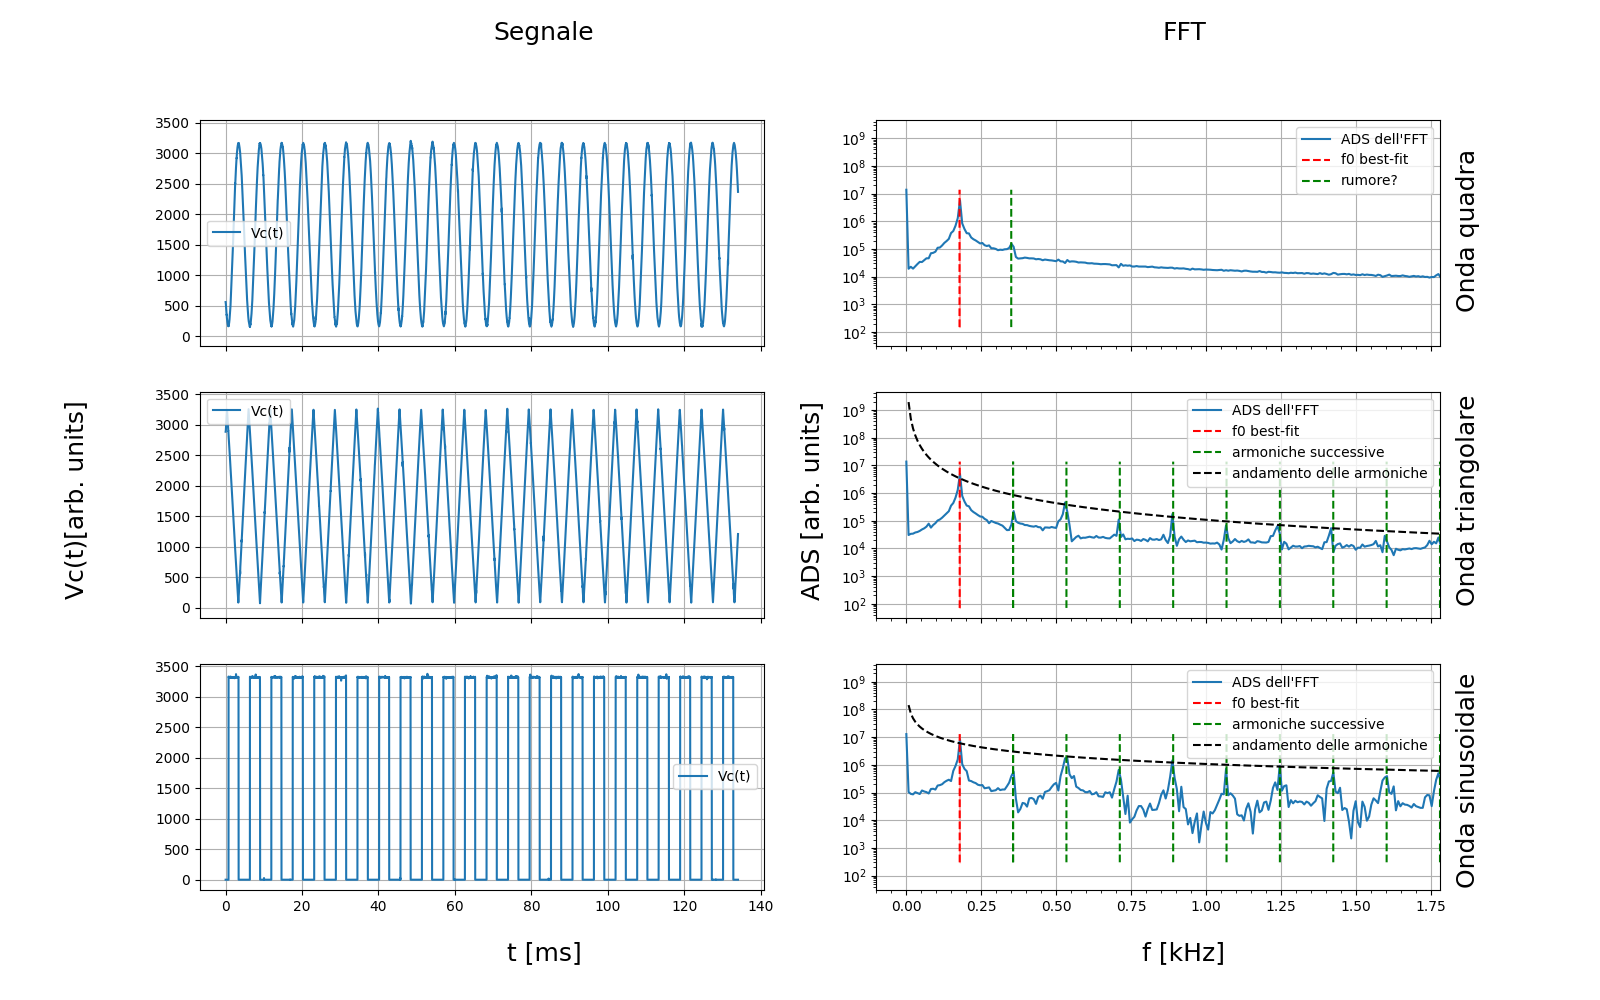
\includegraphics[scale=0.45]{FFT5/FFTwaveforms1.png}
            \caption{Confronto tra le frequenze stimate tramite FFT e bestfit.
                    Attorno ai valori medi è stata rappresentata la barra di errore 
                    con un'area colorata.
                    Coerentemente con quanto ci si può aspettare sono presenti due picchi nella FFT,
                    uno a frequenza nulla, in quanto il segnale non è alternato, l'altro
                    alla frequenza di oscillazione del segnale.}
            \label{fig:for_ond}
        \end{figure}    

    Nel caso dell'onda sinusoidale si osseva la comparsa di un picco dovuto probabilemte
    a rumore a $300$ Hz.
    Per le altre forme d'onda è interessante notare la comparsa delle 
    armoniche successive alla principale, come ci si aspetta dallo 
    sviluppo in serie di seni e coseni delle rispettive forme d'onda.
    In questi casi è stata diseganta sopra la FFT
    la legge di potenza di come scalano le armoniche successive , rispettivamente
    $\frac{1}{k}$ e $\frac{1}{k^2}$ per l'onda quadra e  per quella triangolare.

    E' stato eseguito un bestfit con forma d'onda sinusoidale Eq.(\ref{eq:sin}) 
    per le frequenze principali $f_0$, i risultati 
    sono riportati in Tab.($\ref{tab:for_ond}$) e 
    mostrati in Fig.($\ref{fig:for_ond}$) assieme al rispettivo valore 
    estrapolato dalla FFT.
    E' stata usata la forma d'onda sinusoidale  per tutti i set di dati
    in quanto l'unico obbiettivo del bestfit
    è quello di individuare la frequenza delle oscillazioni.


        \begin{equation}
            f(t; A, \omega, \phi, c) = A \sin{(\omega t + \phi)} + c,
            \label{eq:sin}
        \end{equation}

    Come incertezza sulla frequenza $f_0$ estrapolata dalla FFT è stata 
    considerata la deviazione standard di una distribuzione uniforme attorno
    a $f_0$ con ampiezza la risoluzione del campionamento.  
         

        \begin{table}[H]
            \centering
                \begin{tabular}{ccc}
                    Forma d'onda    &   $f_{0fft}$[kHz]                     & $f_{0bestfit}$[kHz] \\
                    \hline
                    Sinusoide       &   $0.179 \pm 0.001$           & $0.177455 \pm 0.000002$ \\
                    Triangolare     &   $0.179 \pm 0.001$           & $0.1780571\pm 0.0000009$ \\
                    Quadra          &   $0.179 \pm 0.001$           & $0.1780571 \pm 0.0000009$ \\
                \end{tabular}
                \caption{Tutti i valori, eccetto quelli relativi alla sinusoide,
                        sono compatibili tra loro entro le barre di errore. }
                \label{tab:for_ond}
        \end{table}

    Sono state anche fatte acquisizioni "lunghe" di forme d'onda sinusoidali
    e quadrate. Sono riportati i risultati del bestfit in Fig.($\ref{fig:for_lun}$)
    e in Tab.($\ref{tab:for_lun}$).

         

         \begin{figure}[H]
            \centering
            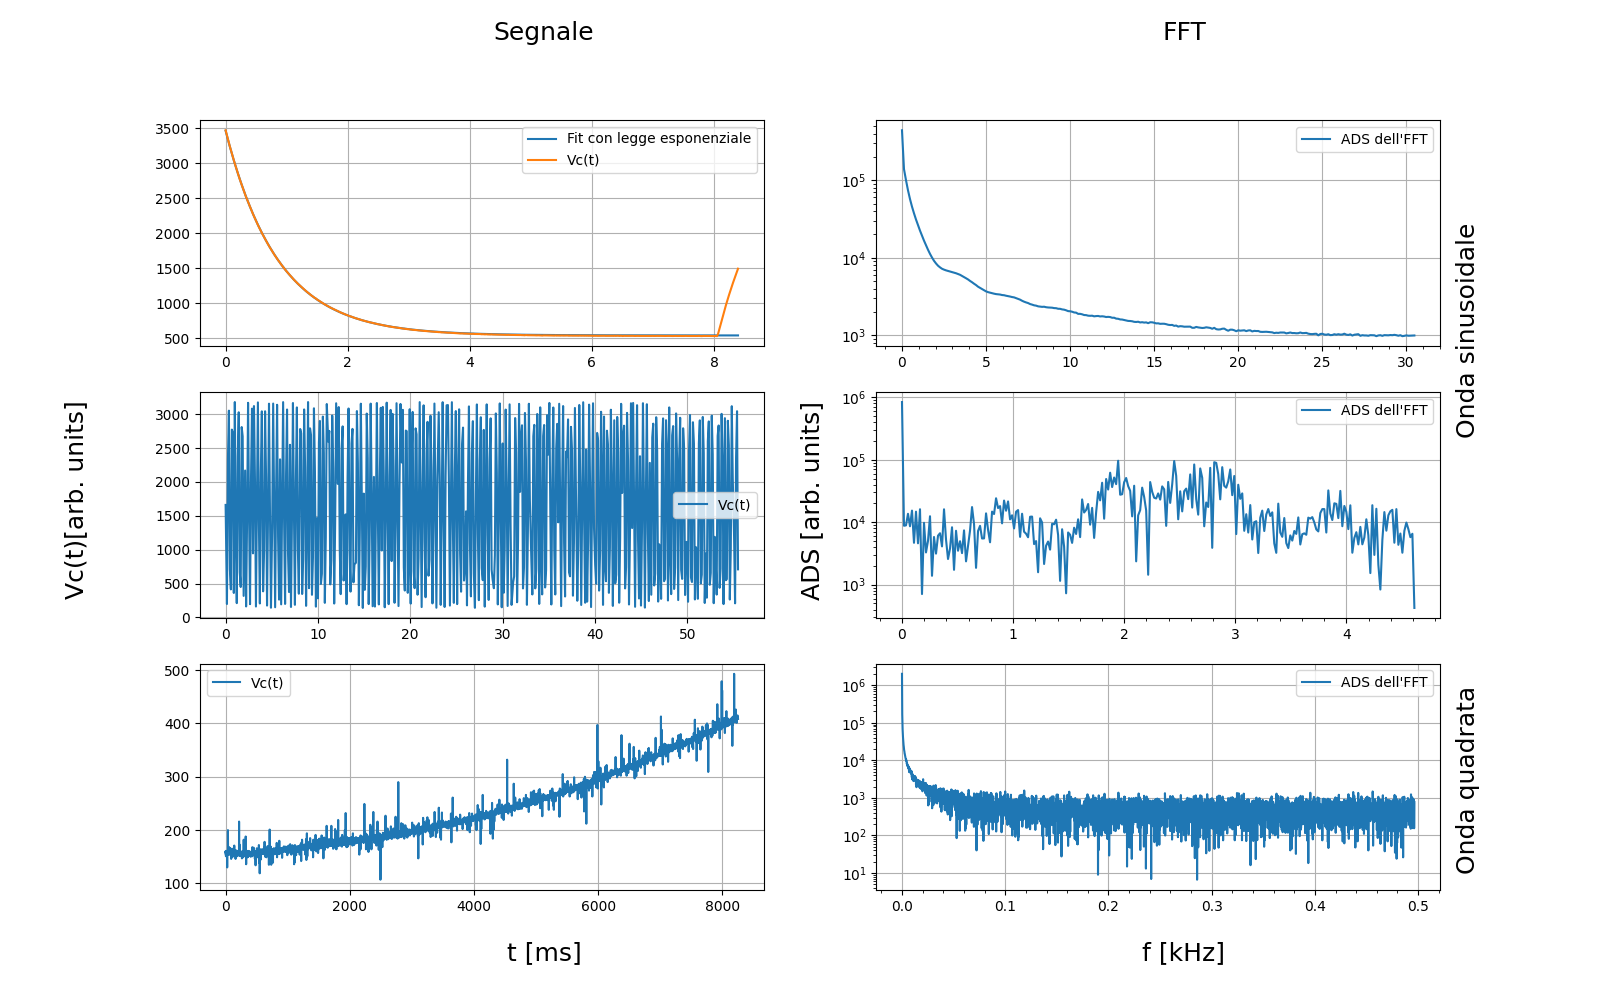
\includegraphics[scale=0.45]{FFT5/FFTwaveforms3.png}
            \caption{A sinistra sono mostrati segnali acquisiti in laboratorio, a destra 
                    è stata eseguita la FFT.
                    E' molto interessante osservare che nel caso dell'onda quadra 
                    non compaiano le armonica successive: questo potrebbe essere 
                    legato al fatto che in media sono presi sette punti per periodo e quindi 
                    è possibile che ci sia un sottocampionamento dei dati per questa analisi.}
            \label{fig:for_lun}
        \end{figure}    


         \begin{table}[H]
            \centering
                \begin{tabular}{ccc}
                    Forma d'onda    &   $f_{0fft}$[kHz]                     & $f_{0bestfit}$[kHz] \\
                    \hline
                    Sinusoide       &   $0.13354 \pm 0.00002$           & $0.13352992 \pm 0.0000003$ \\
                    Quadra          &   $0.13354 \pm 0.00002$           & $0.1334881 \pm  0.000003$ \\
                \end{tabular}
                \caption{Per l'onda sinusoidale la frequenza ricavata dal bestfit è compatibile
                entro la barra di errore con la FFT. Per l'onda quadra questo non si verifica, 
                probabilmente questo è legato al sottocampionamento menzionato nella didascalia 
                di Fig.(\ref{fig:for_lun}).}
                \label{tab:for_lun}
        \end{table}
        


\section{Forme d'onda distorte}

    Sono stati raccolti segnali cambiando il dutycycle  del generatore di funzioni.
    E' stato eseguito un fit con una sinusoide Eq.(\ref{eq:sin}) con l'obbiettivo di
    far convergere solo la frequenza.

    E' stata realizzata per ciascuna forma d'onda l'FFT.
    Come incertezza sulla FFT è stata utilizzata quella discussa in Sez.(\ref{sez:for_ond}).
    Il risultato della manipolazione dei dati è riportato in Fig.($\ref{fig:for_dis}$)
    e in Tab.($\ref{tab:for_dis}$).
        \begin{figure}[H]
                \centering
                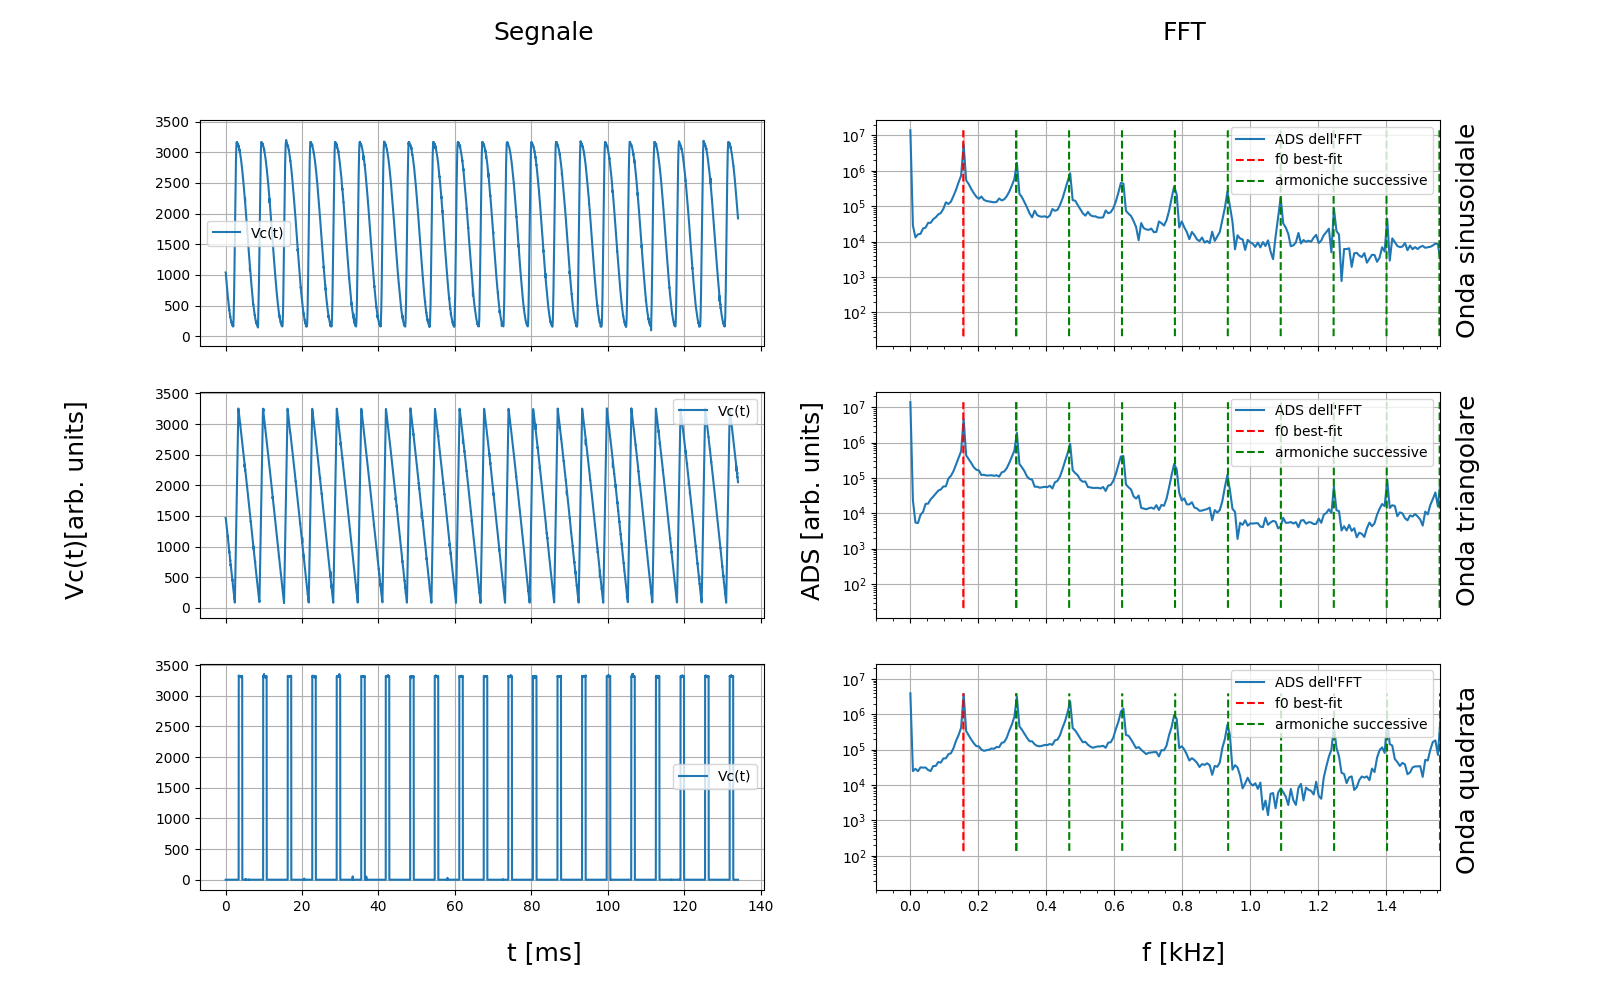
\includegraphics[scale=0.45]{FFT5/FFTwaveforms2.png}
                \caption{A sinistra sono mostrati segnali acquisiti in laboratorio, 
                        a destra è stata eseguita la FFT.
                        Attorno ai valori medi è stata rappresentata la barra di 
                        errore.}
                \label{fig:for_dis}
        \end{figure}   

        \begin{table}[H]
            \centering

                \begin{tabular}{ccc}
                    onda            &   $f_{0fft}$[kHz]                     & $f_{0bestfit}$[kHz] \\
                    \hline
                    Sinusoide       &   $0.156 \pm 0.001$           & $0.15559 \pm 0.00002$ \\
                    Triangolare     &   $0.156 \pm 0.001$           & $0.15559 \pm 0.00002$ \\
                    Quadra          &   $0.156 \pm 0.001$           & $0.15576 \pm 0.00006$ \\
                \end{tabular}
                \caption{I valori del bestfit sono compatibili entro le barre di errore
                con valori ottenuti tramite FFT.}
                \label{tab:for_dis}
        \end{table}
    Si osserva per la comparsa di armoniche successive 
    per la forma d'onda sinusoidale distorta, e la dilatazione per le altre 
    forme d'onda delle ampiezze delle armoniche successive rispetto
    a quelle osservate nei segnali non distorti.

\section{Cattive acquisizioni}

    In Fig.($\ref{fig:merda}$) sono riportati esempi di "cattive acquisizioni".

        \begin{figure}[H]
            \centering
            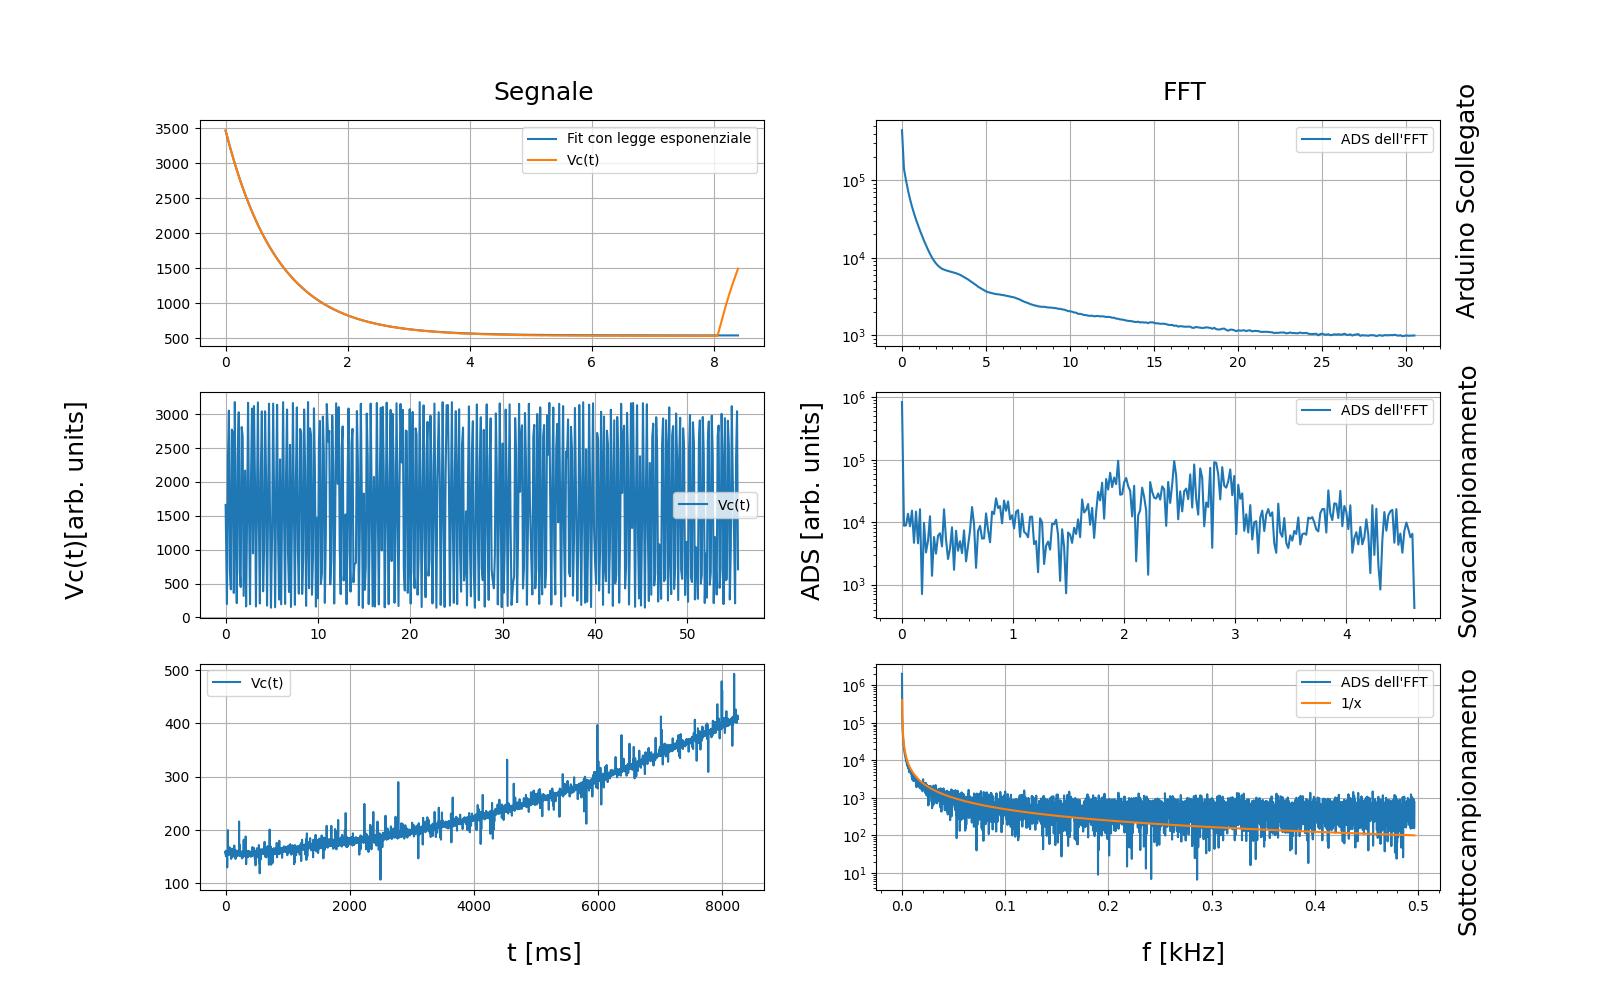
\includegraphics[scale=0.45]{FFT5/FFTwaveforms4.png}
            \caption{I primi due grafici rappresentano il campionamento di una porta di arduino scollegata.
            In mezzo è riporato un sottocampionamento: per ogni periodo è acquisito un 
            solo punto.
            La terza coppia di figure dall'alto rappresenta un sovracampionamento 
            di un periodo: l'acquizione prende  solo il ramo crescente di un seno.}
            \label{fig:merda}
        \end{figure}  
    
    E' stato eseguito un bestfit con una legge esponenziale Eq.(\ref{eq:exp}) per la sezione decrescente
    del segnale acquisito con arduino scollegato: fisicamente questo è legato all'ipotesi 
    che una certa carica presente prima dell'acquisizione 
    sulla porta è dissipata quando la porta comunica con il resto di Arduino.
    
        \begin{equation}
            y=A e^{-\frac{t}{\tau}}+c
            \label{eq:exp}
        \end{equation}
    
    Il risultato del bestfit è riporatto in Tab.($\ref{tab:merda}$)
    

        \begin{table}[H]
            \centering
            \begin{tabular}{cc}
                $\tau[ms]$ & $\chi^2_{norm}$\\
                \hline
                $0.8598\pm0.0004$ &$5$\\
            \end{tabular}
        \caption{Risultati bestfit per legge esponenziale di un'acquisizione 
                con arduino scollegato. $\tau$ è il tempo di decadimento della legge 
                esponenziale Eq.(\ref{eq:exp}).}
        \label{tab:merda}
        \end{table}



    Per quanto riguarda il sovracampionamento è sufficente dire che la 
    FFT non riesce a trovare l'armonica principale del segnale sinusoidale e 
    che i diversi picchi che compaiono nel segnale possono essere di natura puramente
    accidentale.

    Nel caso di sottocampionamento siccome una sinusoide localmente può 
    essere approssimata con una retta, si è disegnato sopra la FFT la funzione
    $\frac{\alpha}{f}$ -dove $\alpha$ è una costante arbitraria-
    in quanto ciascun termine dello sviluppo in serie  di 
    armoniche della funzione $g(f)=f$ è proporzionale all'inverso della 
    corrispettiva frequenza.







\section{Autoscillatore}

    Sono state prese delle misure di un segnale in uscita da un autoscillatore, il cui schema è riportato in Fig(\ref{fig:circuitino_oscillante})
        \begin{figure}[H]
        \begin{minipage}{0.445\textwidth}
            Per ogni segnale registrato, è stato eseguito il fit ai minimi quadratici con 
            Eq.(\ref{eq:sin}) per individuare la frequenza dell'oscillazione sinusoidale 
            del segnale in uscita.
            E' stata eseguita una FFT, e la frequenza del bestfit  è stata confrontata con 
            quella ottenuta dalla FFT.
        \end{minipage}
        \hfill
        \begin{minipage}{0.45\textwidth}
            \centering
            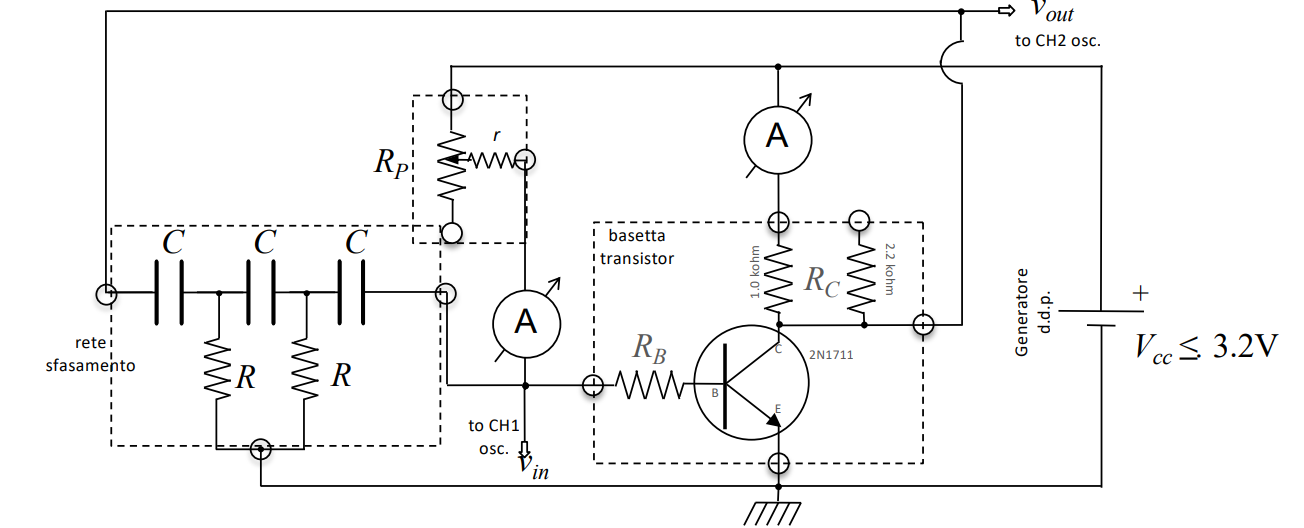
\includegraphics[width=\textwidth]{FFT11/schema_circuitino.png}
            \caption{Schema circuitale dell'oscillatore}
            \label{fig:circuitino_oscillante}
        \end{minipage}
        \end{figure}

    Riportiamo in Fig(\ref{fig:sign_rfft_autoscill}) dei grafici di alcuni segnali con
     a sinistra il segnale in uscita e a destra la trasformata di Fourier del segnale.
    Viene disegnata una linea verticale che rappresenta il valore stimato di $f$ del bestfit.
    
        \begin{figure}[H]
            \centering
            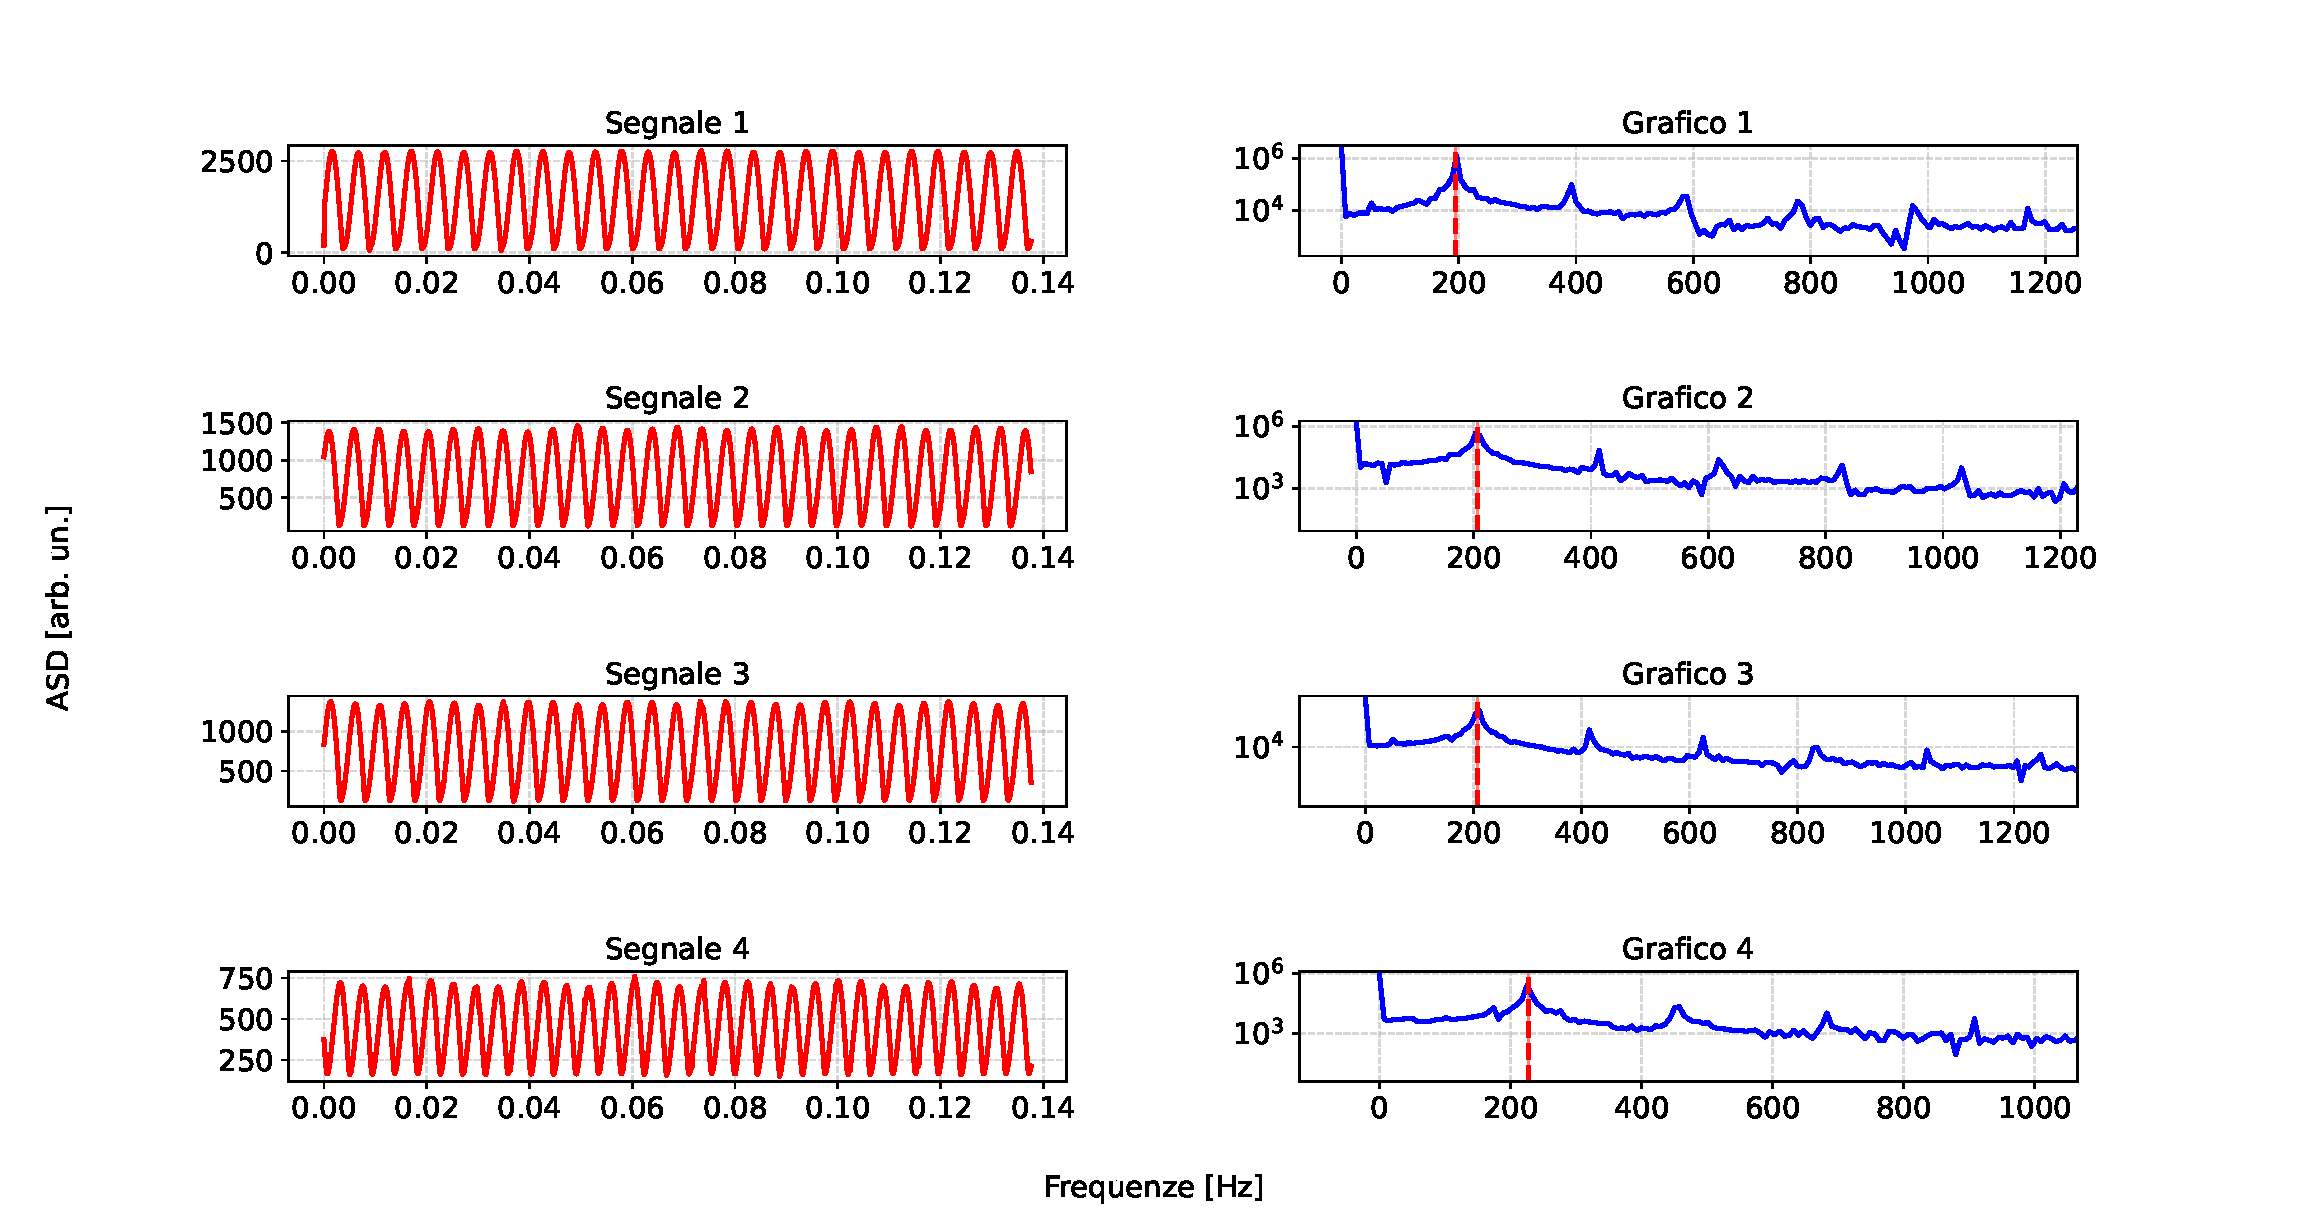
\includegraphics[scale=0.425]{FFT11/first_graph.pdf}
            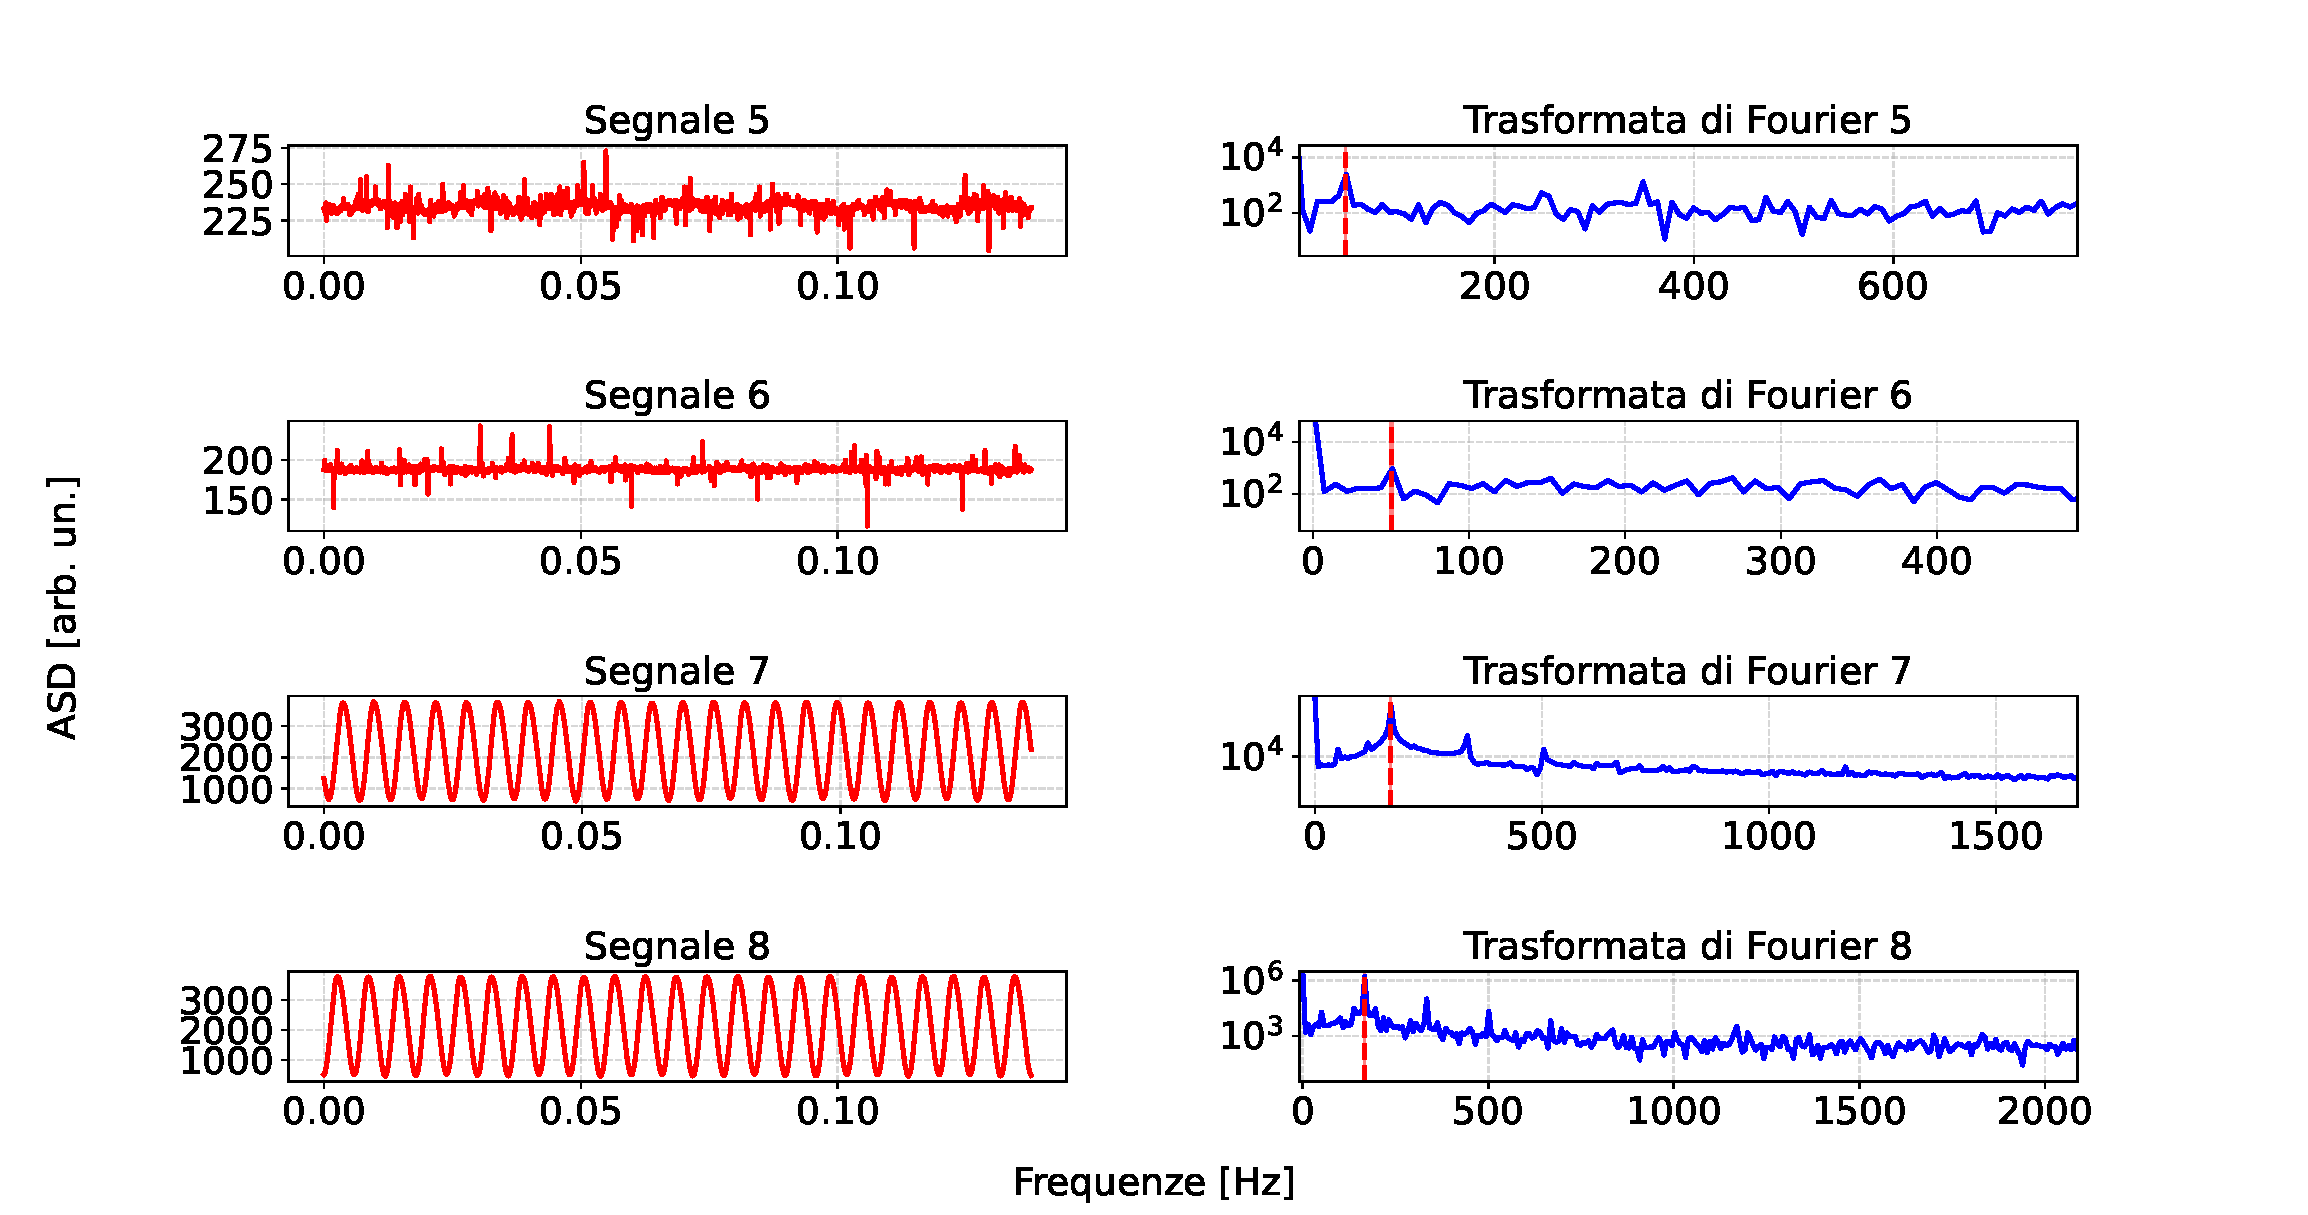
\includegraphics[scale=0.425]{FFT11/second_graph.pdf}
        \end{figure}
            
        \begin{figure}[H]        
            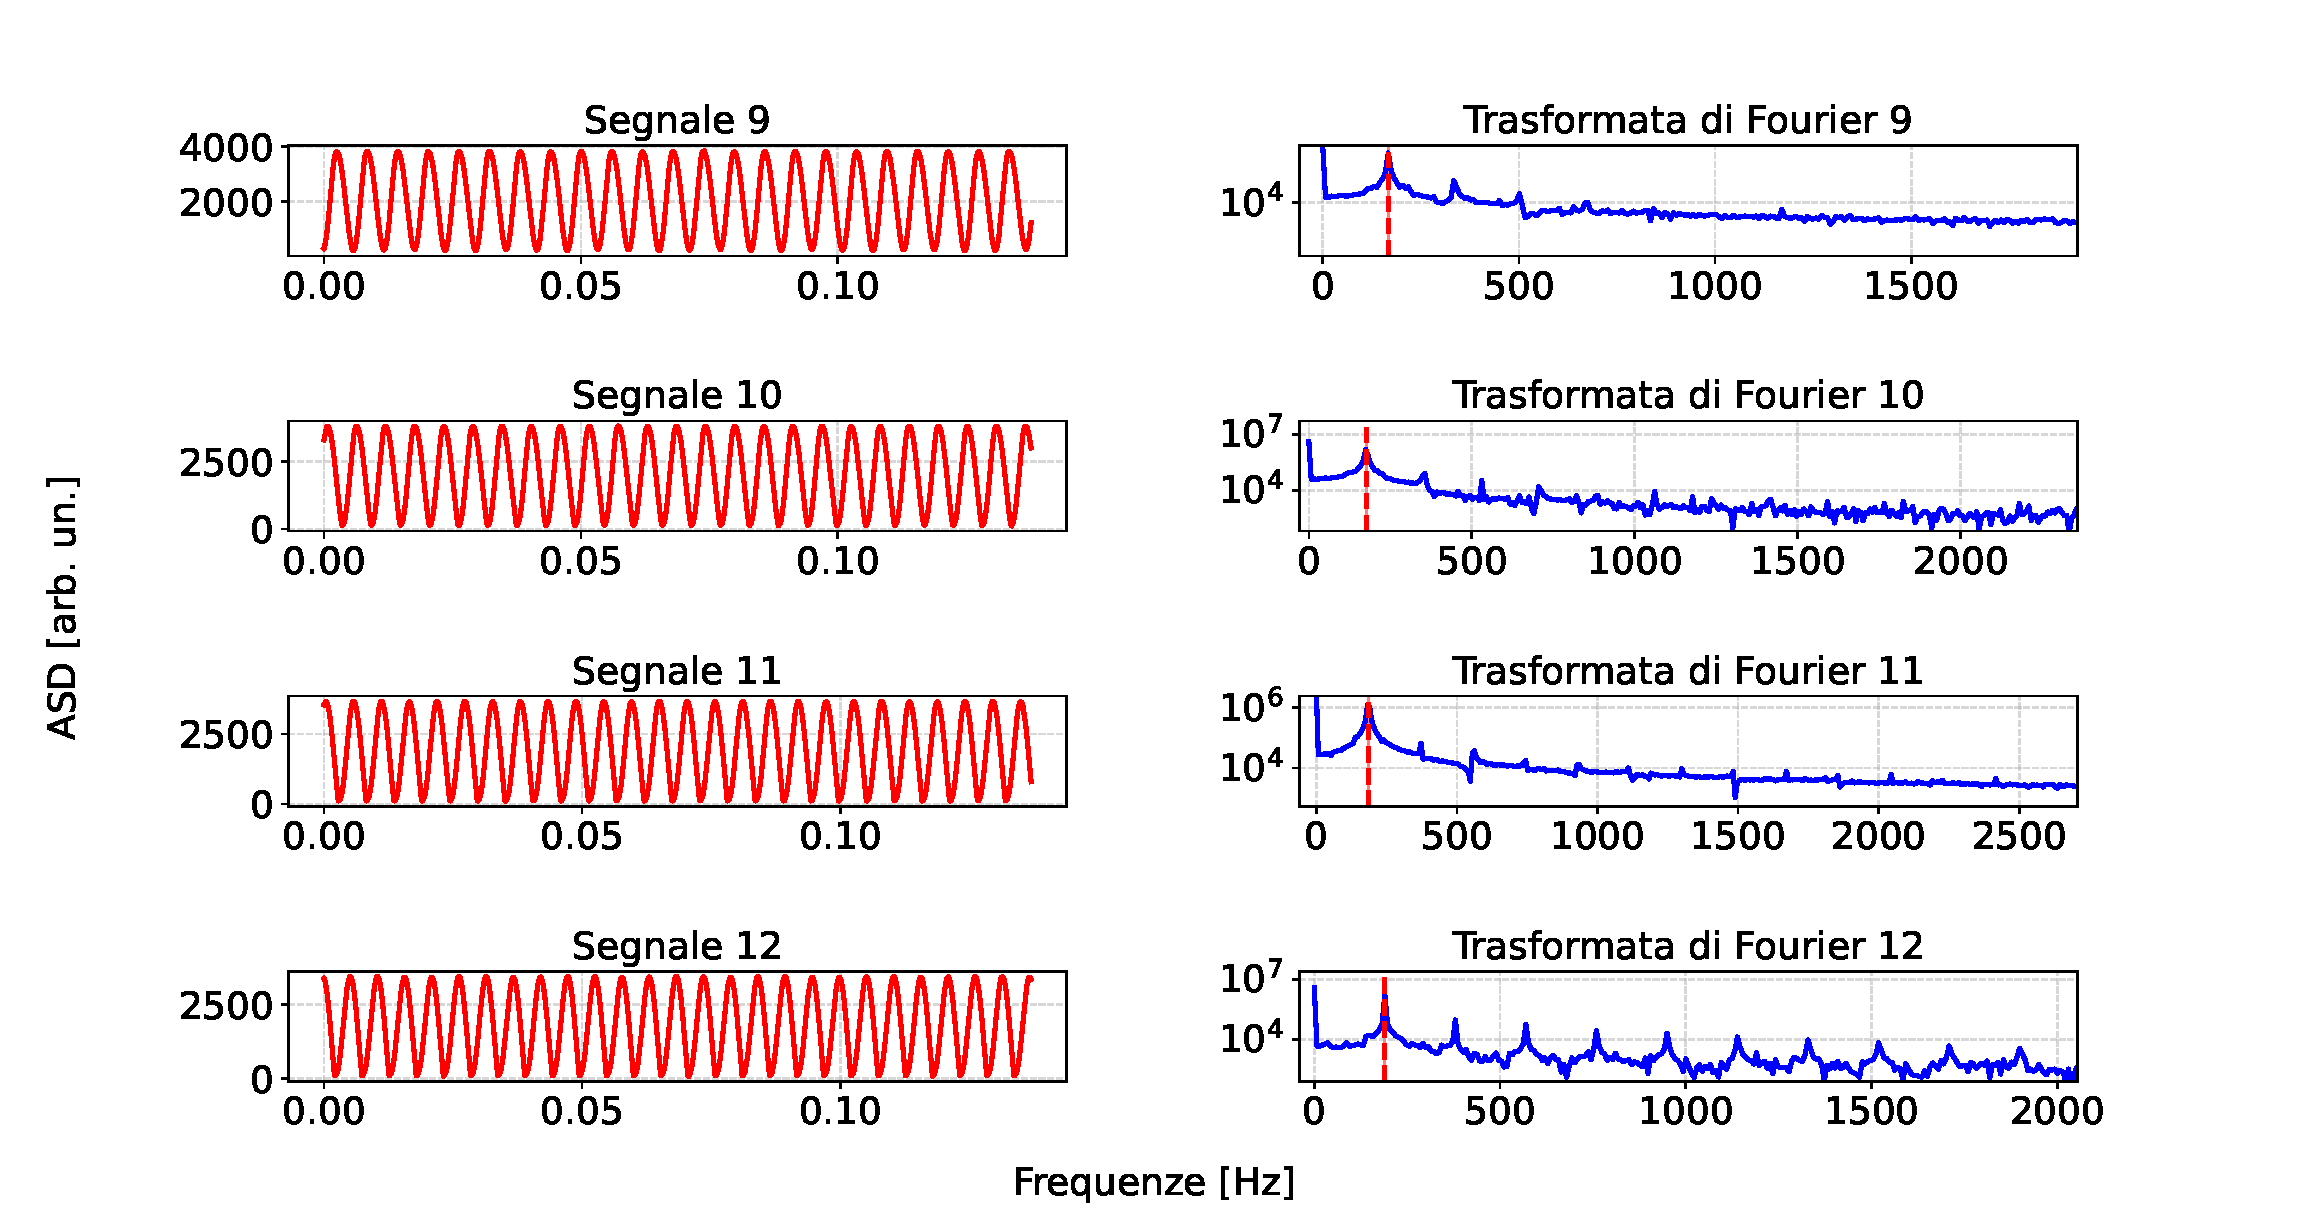
\includegraphics[scale=0.425]{FFT11/third_graph.pdf}
            \caption{Grafici del segnale in uscita dall'autoscillatore (a sinistra) e 
            della sua FFT (a destra). Attorno alla frequenza stimata dal bestfit è 
            rappresentata con un'area l'incertezza.}
            \label{fig:sign_rfft_autoscill}
        \end{figure}

    Ci aspettermmo solo un picco dovuto all'armonica principale in quanto
    l'autoscillatore dovrebbe produrre un segnale sinusoidale.
    Tuttavia ciò non accade per il fatto che l'autoscillatore fa passare più armoniche. 
    Questo è dovuto al fatto che non si tratta di un autoscillatore puro e 
    la funzione di trasferimento ci dà solo l'armonica principale.
    In Tab(\ref{tab:cft_rfft_bestfit}) riportiamo i valori di bestfit.

        \begin{table}[H]
            \centering
            \begin{tabular}{c c c}
                \toprule
                $n$ & $f_{0_\text{FFT}} \, [\text{Hz}]$ & $f_{0_\text{bestfit}} \, [\text{Hz}]$ \\
                \midrule
                1 & $195 \pm 2$         & $195.13 \pm 0.06$ \\
                2 & $203 \pm 2$       & $206.61 \pm 0.07$ \\
                3 & $210 \pm 2$         & $207.86 \pm 0.07$ \\
                4 & $225 \pm 2$         & $227.02 \pm 0.08$ \\
                5 & $50 \pm 2$          & $50 \pm 1$ \\
                6 & $50 \pm 2$          & $50 \pm 4$ \\
                \bottomrule
            \end{tabular}
            \caption{Tabella con i valori di frequenza del segnale stimata tramite FFT 
            e tramite bestfit. Il segnale 5 e il segnale 6 sono interessanti
            in quanto sono soggetti a rumore: l'incertezza dell'FFT non scala col rumore ma con
            la lunghezza dell'acquisizione, invece il bestfit risente pesantemente della qualità dei dati.}
            \label{tab:cft_rfft_bestfit}
        \end{table}
    Si osserva che i valori di frequenza stimati tramite bestfit e tramite FFT 
    sono compatibili entro le barre di errori per tutti i valori. 
    Come incertezza sulla FFT è stata utilizzata quella discussa in Sez.(\ref{sez:for_ond}).

\section{Oscillazioni smorzate}

        
        \begin{figure}[H]
            \begin{minipage}{0.45\textwidth}
                Sono state prese delle misure di segnale in uscita da un circuito RLC,
                come mostrato in Fig($\ref{fig:osc_diag}$) per tre diversi condensatori.
                Sono stati misurati il periodo e la frequenza delle oscillazioni.
                E' stato eseguito un fit ai minimi quadrati per un'oscillazione 
                smorzata per determinarne il periodo con Eq.(\ref{eq:sin}).
                E' stata eseguita una FFT per il medesimo scopo.
                I risultati sono riportati in Tab.($\ref{tab:osc_smor}$) e 
                in Fig.($\ref{fig:osc_smor}$).
            \end{minipage}%
            \hfill
            \begin{minipage}{0.45\textwidth}
                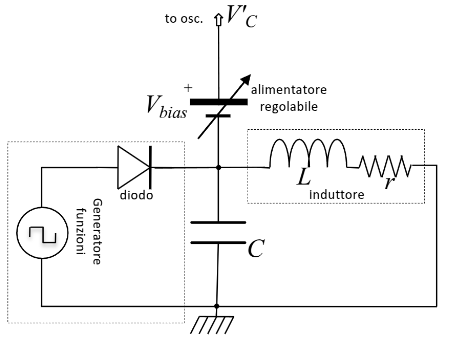
\includegraphics[width=\textwidth]{FFT12/RLCdiagram.png}
                \caption{Diagramma del circuito RLC realizzato.}
                \label{fig:osc_diag}
            \end{minipage}
        \end{figure}

        \begin{figure}[H]
            \centering
            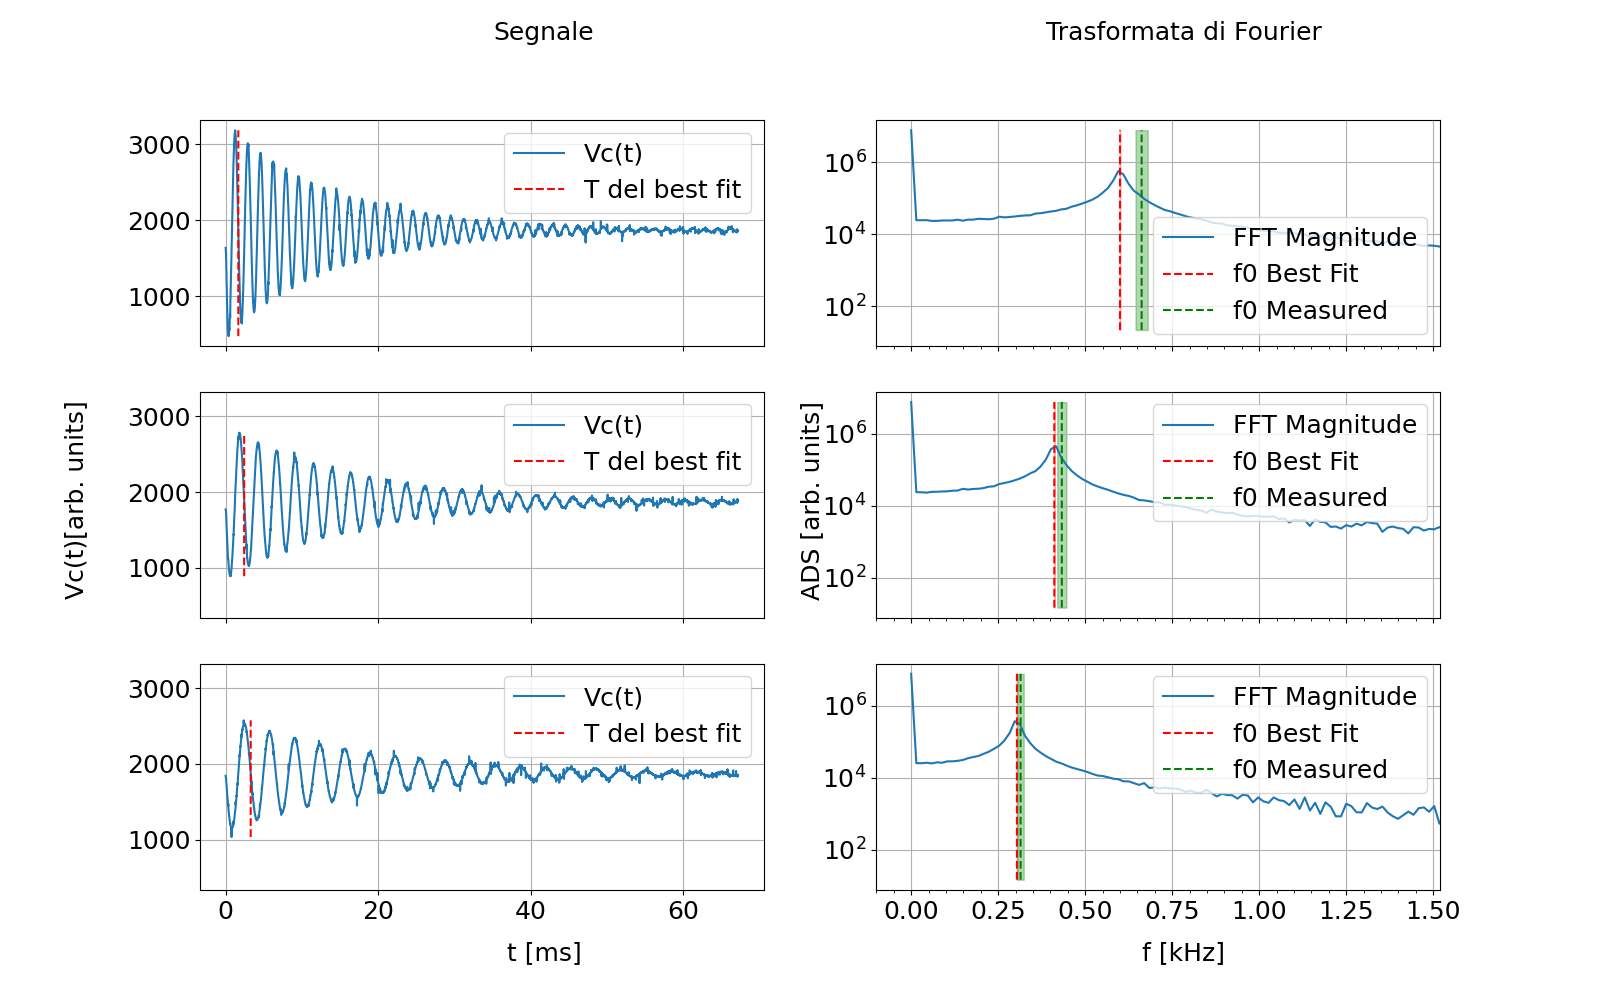
\includegraphics[width=\textwidth]{FFT12/FFTRLC.png}
            \caption{A sinistra è rappresentato il segnale. A destra è rappresentata la FFT insieme
            alla frequenza stimata dal bestfit e quella misurata in laboratorio.
            Le incertezze su queste due grandezze sono rappresentate con due rispettive aree colorate.
            }
            \label{fig:osc_smor}
        \end{figure}

        \begin{table}[H]
            \centering
            
                \begin{tabular}{cccc}
                    $C$[$\mu$F]          &$f_{0mis}$                &   $f_{0fft}$[kHz]       & $f_{0bestfit}$[kHz] \\
                    \hline
                    $0.1 \pm 20\%tol.$   &     $0.66 \pm 0.02$      & $0.595 \pm 0.004$       & $0.6001 \pm 0.0003$ \\
                    $0.22 \pm 20\%tol.$  &$0.43 \pm 0.01$           & $0.416 \pm 0.004$       & $0.41131\pm 0.00002$ \\
                    $0.47 \pm 20\%tol.$  &$0.314 \pm 0.009 $        &$0.298 \pm 0.004$        & $0.30393\pm 0.00002$ \\
                \end{tabular}
                \caption{Confronto tra le frequenze di oscillazione misurate 
                con quelle ottenute tramite FFT e bestfit.}
                \label{tab:osc_smor}
        \end{table}
    
    Tutte le frequenze sono compatibili eccetto nel primo caso per la frequenza 
    misurata.

    Siccome il segnale non è perfettamente sinusoidale, la FFT
    presenta un ampio spettro di armoniche attorno al picco principale.

\section{Materiali nel core dell'induttore}
        \begin{figure}[H]
            \begin{minipage}{0.45\textwidth}
                Sono state prese delle misure di segnale in uscita da un circuito RLC,
                come mostrato in Fig($\ref{fig:mat_diag}$) inserendo diversi materiali dentro 
                il core dell'induttore.
                E' stato eseguito un fit ai minimi quadrati per un'oscillazione 
                smorzata Eq.(\ref{eq:osc_smorz}) per determinarne il periodo e il tempo di smorzamento.
                E' stata eseguita una FFT per determinare il periodo di oscillazione.
                I risultati sono riportati in Tab.($\ref{tab:mat_smor}$) e 
                in Fig.($\ref{fig:mat_smor}$).
            \end{minipage}
            \hfill
            \begin{minipage}{0.45\textwidth}
                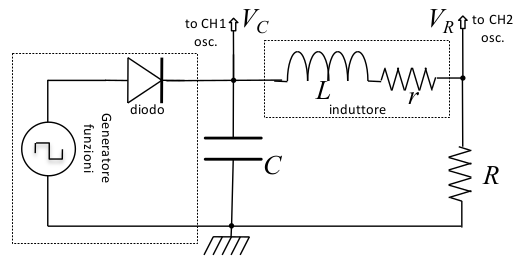
\includegraphics[width=\textwidth]{FFT13/RLCmaterialsdiagram.png}
                \caption{Diagramma del circuito RLC realizzato.}
                \label{fig:mat_diag}
            \end{minipage}
        \end{figure}

        \begin{equation}
            y=A e^{-t/\tau} \sin(2 \pi f_0 t + phi) +c
            \label{eq:osc_smorz}
        \end{equation}

        \begin{figure}[H]
            \centering
            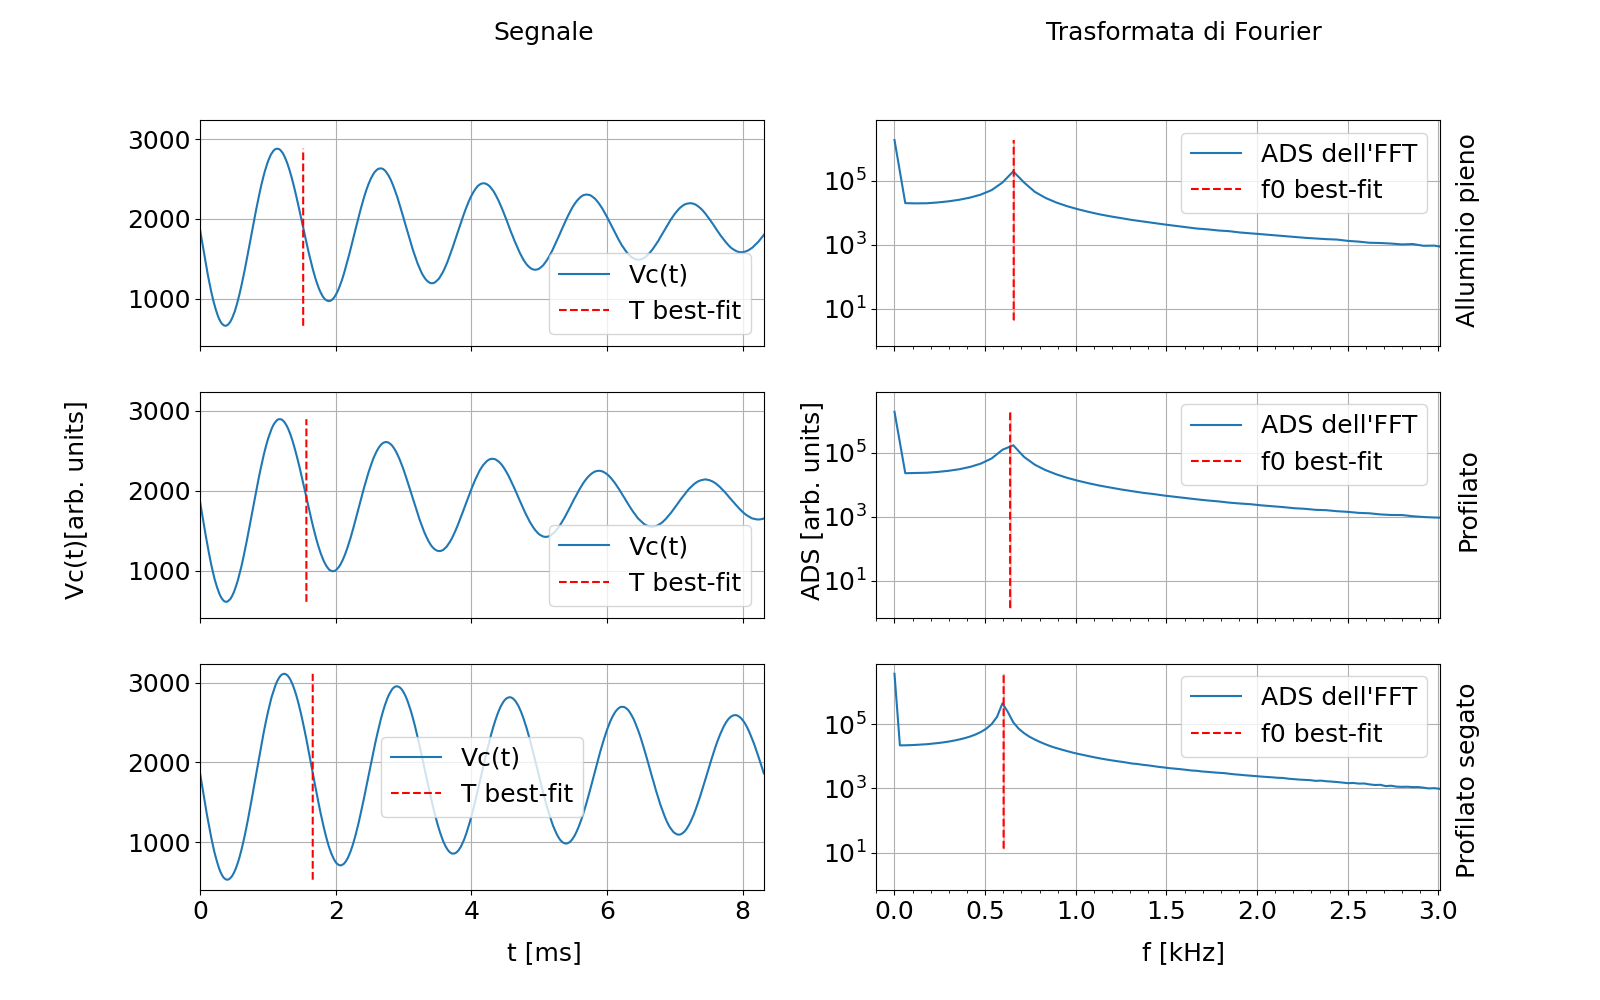
\includegraphics[width=\textwidth]{FFT13/FFTMATERIALS1.png}
        \end{figure}

        \begin{figure}[H]
            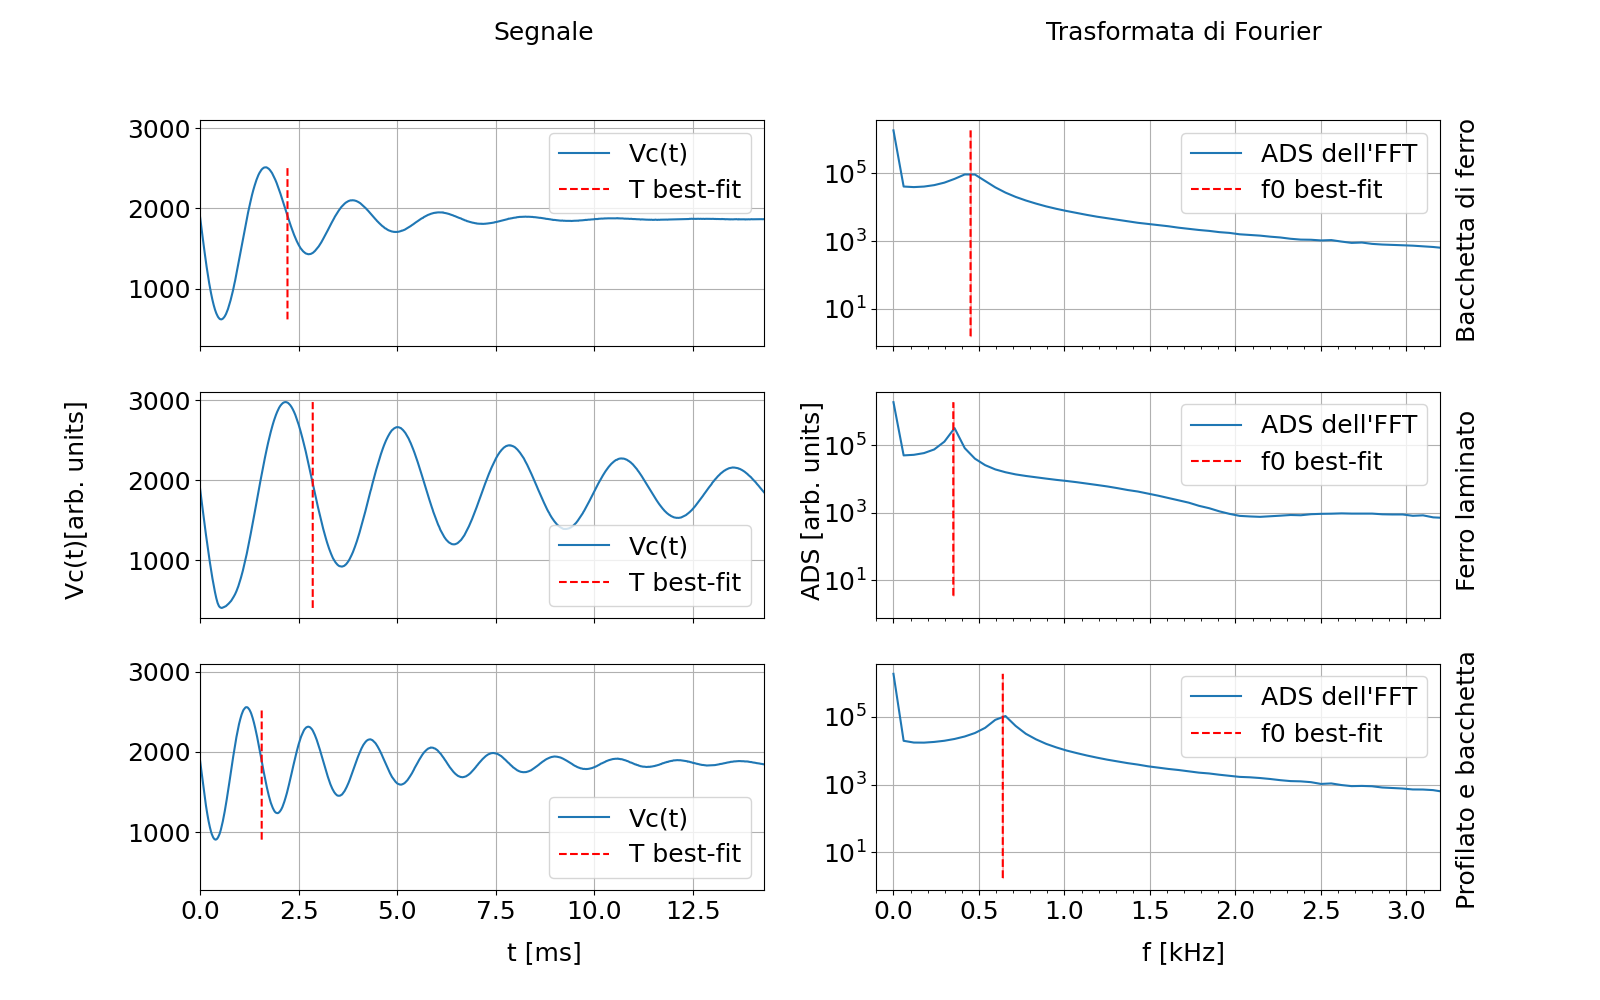
\includegraphics[width=\textwidth]{FFT13/FFTMATERIALS2.png}
            \caption{Confronto tra le frequenze di oscillazione misurate con quelle ottenute tramite FFT e bestfit.
            Attorno ai valori medi è stata rappresentata la barra di errore per il valore
            misurato e per quello del bestfit, per il quale non si vede essendo molto piccola.}
            \label{fig:mat_smor}
        \end{figure}

        \begin{table}[H]
            \centering
            \caption{Confronto tra le frequenze di oscillazione misurate con quelle ottenute tramite FFT e bestfit.}
                \begin{tabular}{ccc}
                    materiale           &   $f_{0fft}$[kHz]     & $f_{0bestfit}$[kHz] \\
                    \hline
                    Alluminio pieno     & $0.65\pm0.02$         & $0.657\pm0.008$ \\
                    Profilato           & $0.65\pm0.02$         & $0.637\pm0.008$ \\
                    Profilato segato    & $0.595\pm0.009$       & $0.601\pm0.002$ \\
                    Bacchetta di ferro  & $0.42\pm0.02$         & $0.451\pm0.009$ \\
                    Ferro laminato      & $0.35\pm0.02$         & $0.349\pm0.009$ \\
                    Profilato e bacchetta& $0.65\pm0.02$        & $0.639\pm0.009$ \\  
                \end{tabular}
                \label{tab:mat_smor}

        \end{table}

        Le frequenze ottenute tramite la FFT e tramite il bestfit sono compatibili, 
        eccetto per la bacchetta di ferro, entro la barra di errore.
        Il problema con la bacchetta di ferro è che essendo il segnale molto smorzato, 
        il picco non è molto pronunciato; in aggiunta siccome l'acquisizione non è stato
        possibile prenderla suffiecienemente lunga -in quanto il segnale sarebbe stato 
        eccessivamente soppresso-, si sovrappone al problema precedente 
        uno legato alla scarsa risoluzione dei punti nello spettro delle frequenze.

        
        Si può osservare che per il blocco di alluminio pieno e il profilato di alluminio,
        il periodo di oscillazione diminuisce, in quanto l'alluminio è diamagnetico, 
        e il periodo è inversamente proporzionale all'induttanza, la quale diminuisce.
        
        Analogamente per il ferro laminato e, in maggior misura, per la bacchetta di 
        ferro il periodo di oscillazione aumenta per il comportamento da ferromagnete.
        
        Nella discussione appena fatta sto trascurando il contributo dato dal 
        tempo caratterstico di smorzamento al periodo di oscillazione.
        
        Il tempo caratteristico di smorzamento è rilevante nei grafici 
        delle FFT, Fig($\ref{fig:mat_smor}$), in quanto impone l'ampiezza del picco:
        si osserva che questo aumenta per ogni materiale inserito nel core 
        rispetto a quanto visto nel caso  del vuoto a Fig.($\ref{fig:osc_smor}$).
        Tuttavia questo non accade per il profilato segato dove, è possibile  
        aspettarsi che gli effetti delle correnti parassite siano meno importanti.

        





\section{"Il pinnacolone"}
    Per il circuito in Fig.(\ref{fig:mat_diag}) è stato simulato il transiente nel quale 
    il diodo torna dall'interdizione nella quale avvengono le oscillazioni alla conduzione.
    Per determinare $Vc$ la grandezza rilevante è la corrente che passa per il 
    ramo dell'induttore: è stata dunque usata un'onda quadra a cui è stata applicata la 
    funzione di trasferimento in Eq.(\ref{eq:tran1}).
    Il transiente è osservato dall'oscilloscopio in DC, in tal caso il segnale non viene 
    deformato, o in AC dove alla funzione di trasferimento in Eq.(\ref{eq:tran1}) si 
    moltiplica quella del filtro passa-alto in Eq.(\ref{eq:osc}).
        \begin{equation}
            T_{osc}(\omega)=\frac{1}{1-\frac{j\omega_{osc}}{\omega}}        
            \label{eq:osc}
        \end{equation}
    
        \begin{equation}
            Z_1=\frac{1}{j \omega C} \quad 
            Z_2= R + r + j \omega L \quad 
            Z=r_{G}+\frac{Z_1 Z_2}{Z_1 +Z_2} \quad 
            I_{\omega L}=\frac{V_{\omega} Z_1}{Z_1 Z + Z_2 Z} 
            \label{eq:tran1}
        \end{equation}
    Oltre agli elementi in Fig.(\ref{fig:mat_diag}) è stata aggiunta $r_{G} = 50 \Omega$ interna al generatore.
    Il risultato della simulazione è riportato in Fig.(\ref{fig:pinnacolone}).

    \begin{figure}[H]
        \centering
        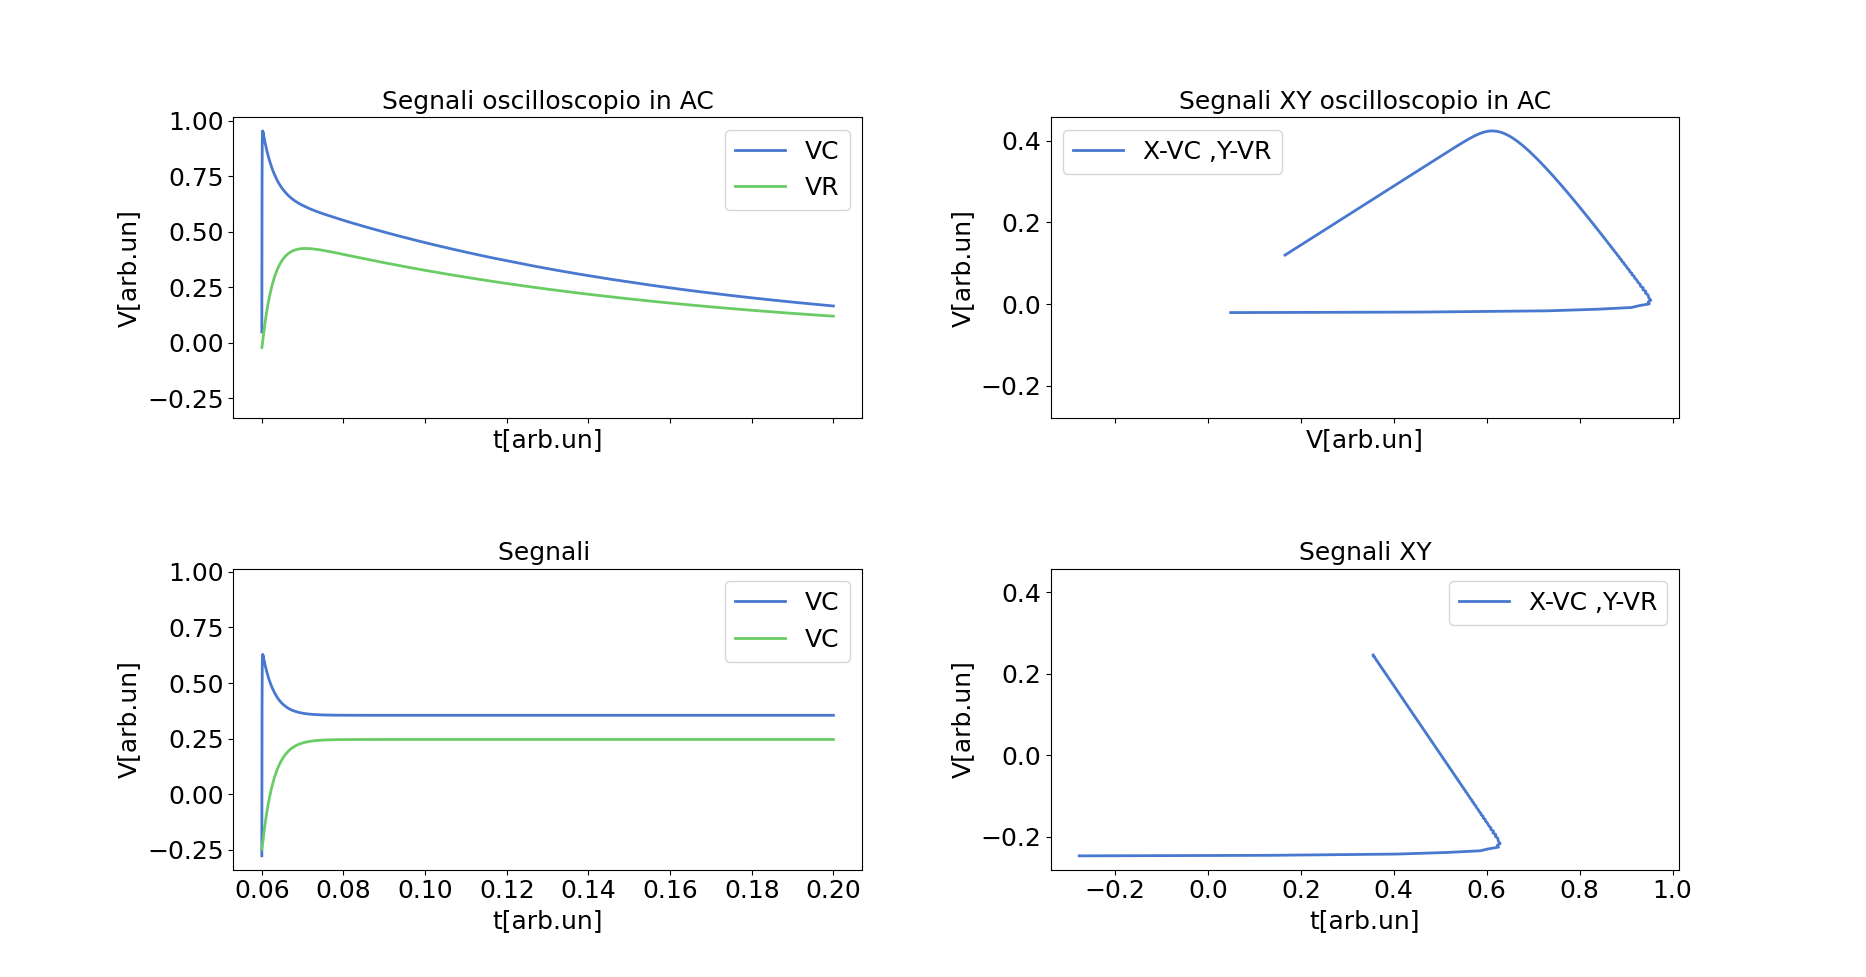
\includegraphics[width=\textwidth]{FFT13/pinnacolone.png}
        \caption{E' stata trovata la forma d'onda desiderata, tuttavia non è stato raccordato il segnale prima 
            e dopo il transiente. Il problema principale è che l'onda quadra trasformata con la funzione di 
            trasferimento non è nulla nel punto di raccordo prima e dopo il transiente
            nonostante lo sia l'onda quadra.}
        \label{fig:pinnacolone}
    \end{figure} 


\section{Glicemia}

        E' stata acquisita la glicemia di un paziente di diabete mellito tipo 1 in 
        due periodi diversi: le vacanze natalizie e la sessione di studio per gli esami.
        I risultati dell'analisi con FFT sono riportati in Fig.($\ref{fig:rubbish}$).
        I due periodi sono paragonabili in quanto ravvicinati e si assume che
        il clima e lo stess non abbiano subito variazioni significative 
        nel paziente.
        Per il periodo di esami  è disponibile un'acquisizione più lunga, i risultati
        della FFT sono  riportati in Fig.(\ref{fig:rubbish1}).
        
        Si evidenziano i tempi che determinano le frequenze caratteristiche dell'andamento glicemico:
            \begin{itemize}
                \item 3 ore - il tempo di effetto dell'insulina.
                \item 6 ore - il tempo che durante il giorno intercorre tra i pasti.
                \item 24 ore - il giorno (da cui il sonno, la produzione ormonale, le attività.
                svolte...)
            \end{itemize}
            \begin{figure}[H]
                \centering
                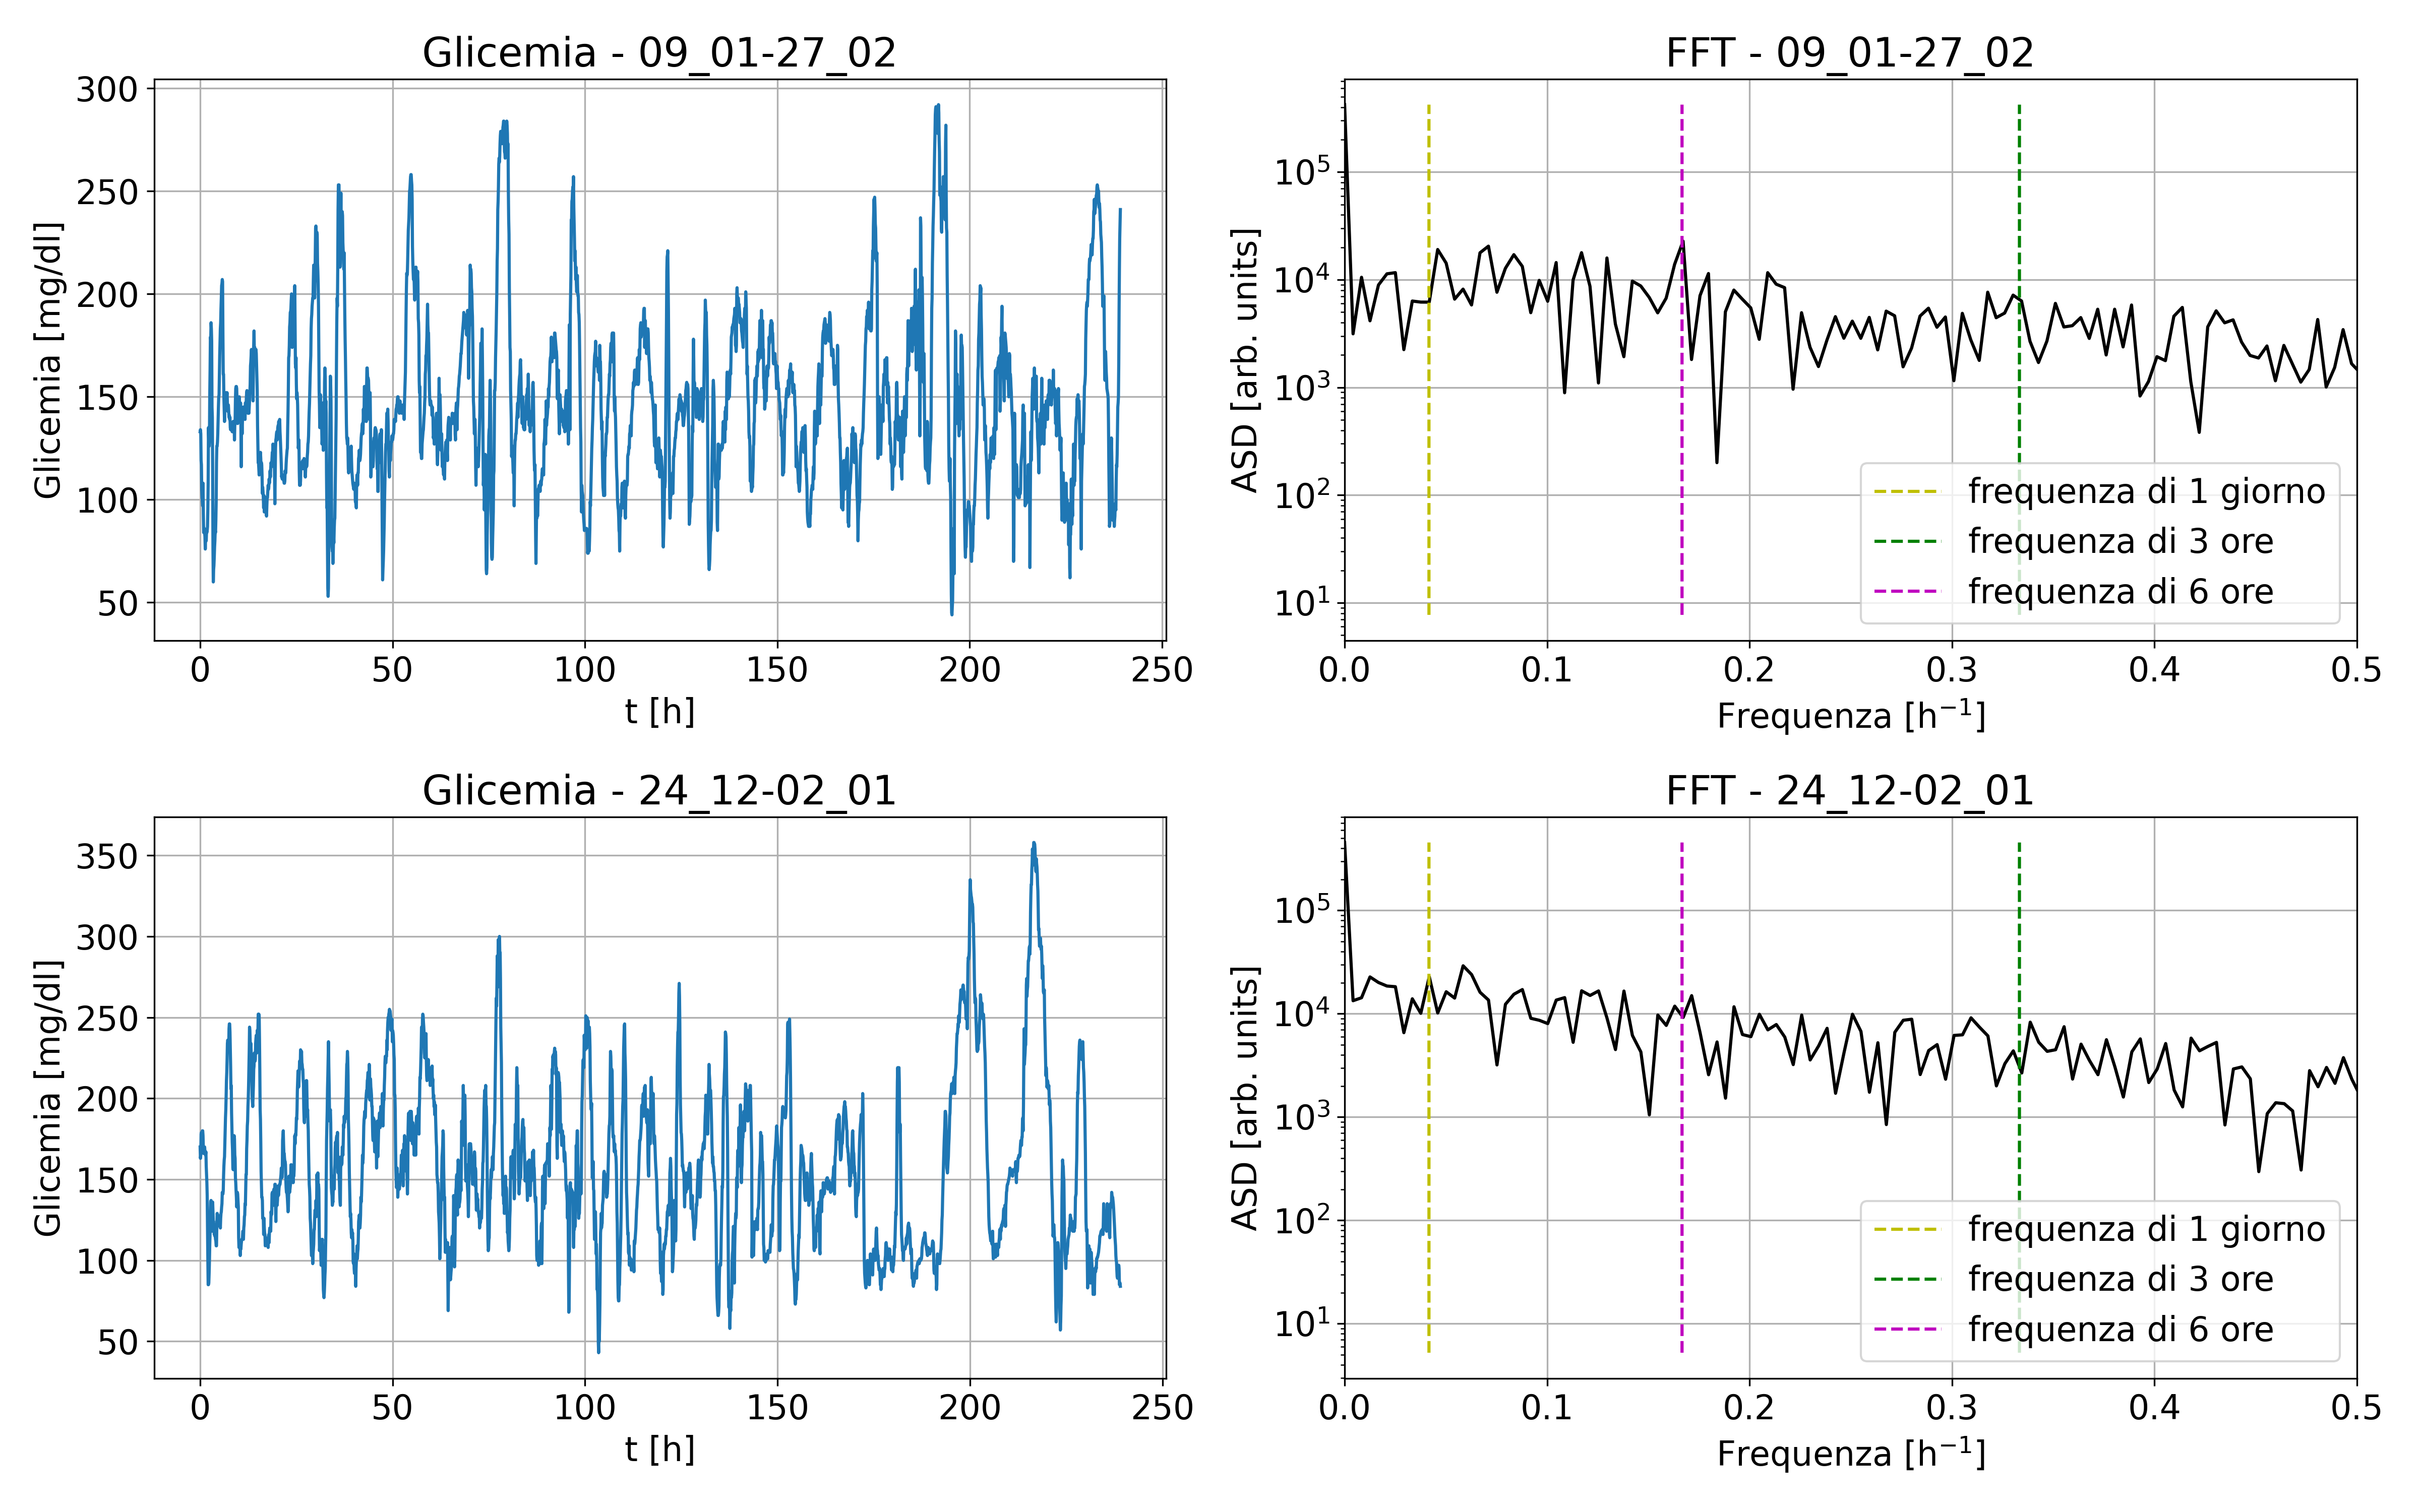
\includegraphics[width=\textwidth]{rubbish/rubbish.png}
                \caption{C'è maggiore regolarità nel 
                periodo di studio rispetto alle festività: il picco legato
                al giorno e quello legato ai pasti scompare durante le festività 
                per probabilemte le persistenti iperglicemie dovute all'aumentata 
                insulino-resistenza e ai pasti più ricchi di grassi.}
                \label{fig:rubbish}
            \end{figure} 

            \begin{figure}[H]
                \centering
                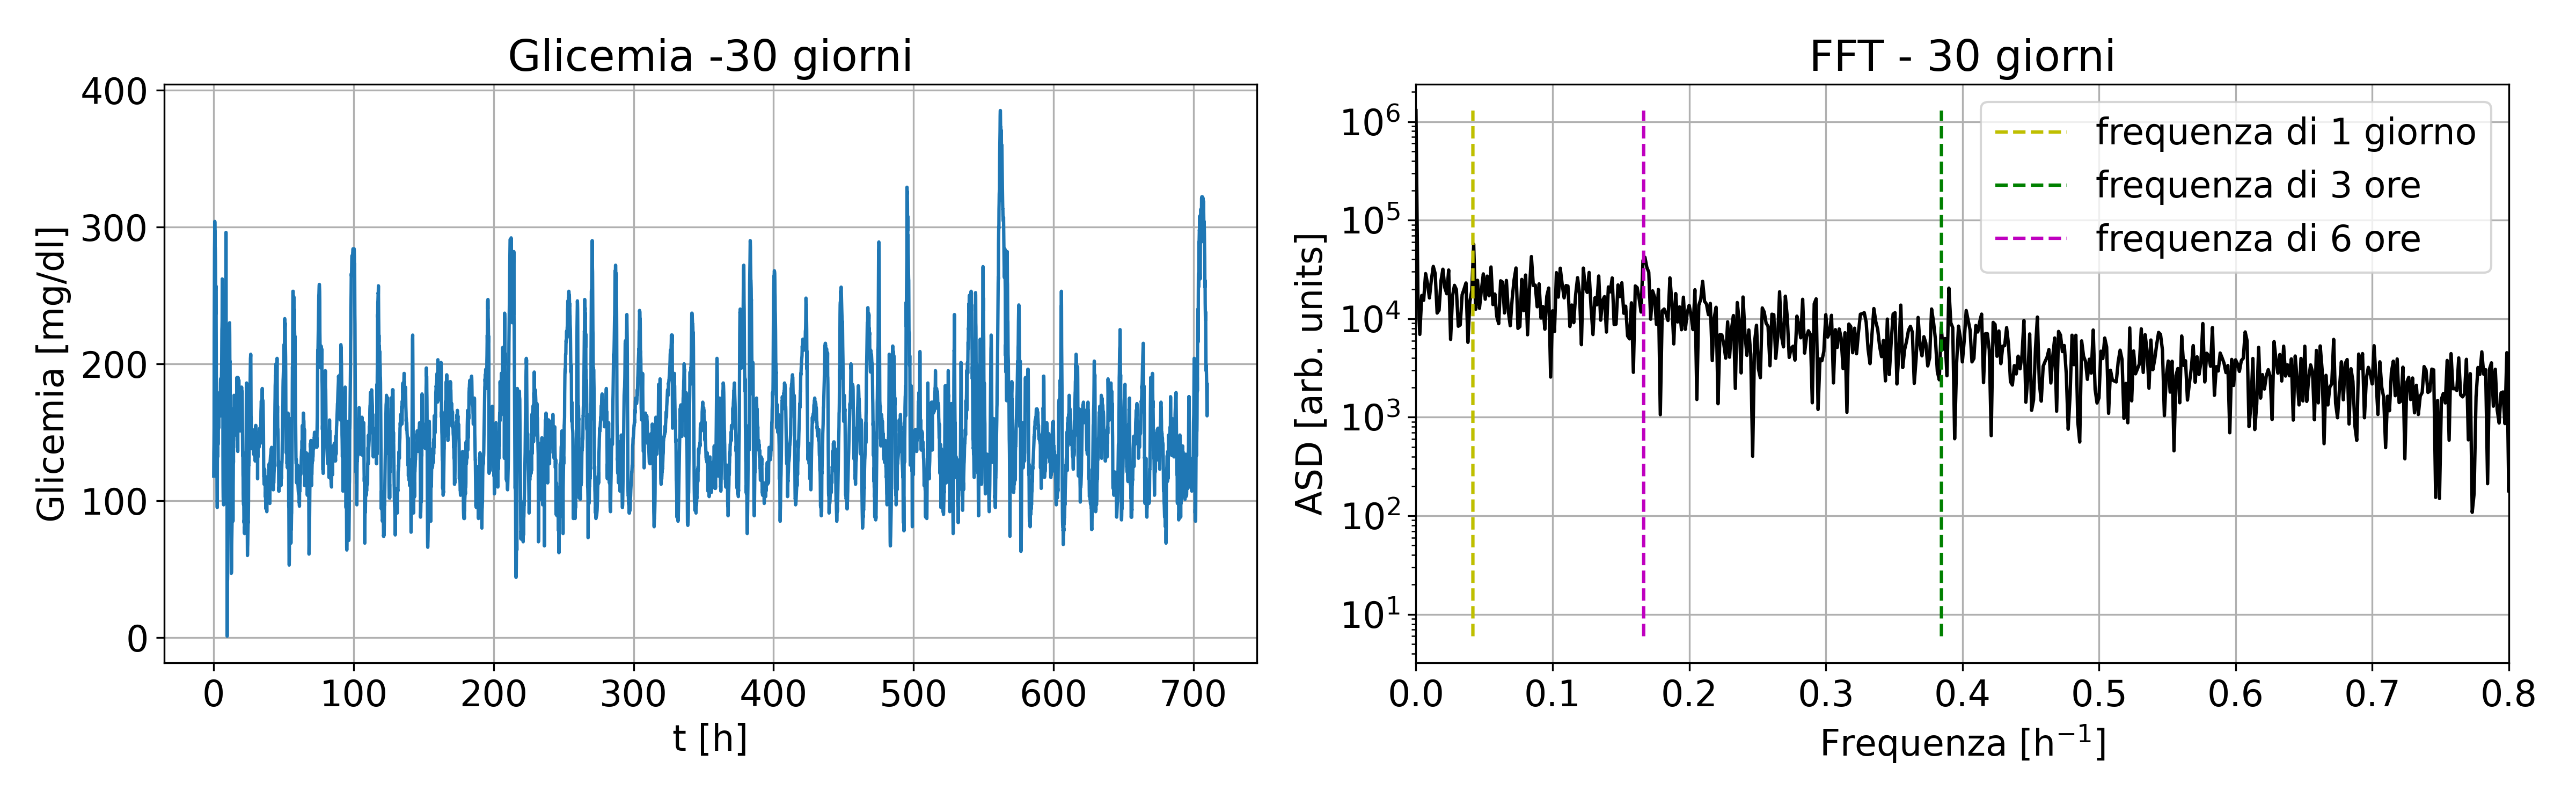
\includegraphics[width=\textwidth]{rubbish/porcheria.png}
                \caption{A sinistra glicemia acquisita in un mese di sessione di studio,
                 a destra l'FFT. Con un intervallo di campionamento più ampio rispetto 
                 a Fig.(\ref{fig:rubbish}) i picchi sono più evidenti.}
                \label{fig:rubbish1}
            \end{figure} 
\end{document}